\documentclass{article}
\usepackage[utf8]{inputenc}
\usepackage[T1]{fontenc}
\usepackage[export]{adjustbox}
\usepackage{mathtools,amsthm,amssymb,icomma,upgreek,xfrac,enumerate, enumitem, bbm,titlesec,lmodern,polski,derivative,multicol,titling,graphicx,url,amsmath,caption,lipsum,float,longtable,booktabs}
\usepackage[table,xcdraw]{xcolor}
\usepackage[hidelinks,breaklinks,pdfusetitle,pdfdisplaydoctitle]{hyperref}
\setlength{\droptitle}{-1cm}
\mathtoolsset{showonlyrefs,mathic}
\title{Proces ryzyka i Ruch Browna}
\author{Adam Wrzesiński, Joanna Kołaczek}
\date{26.06.2022}
\newtheoremstyle{break}
{\topsep}{\topsep}%
{\normalfont}{}%
{\bfseries}{}%
{\newline}{}%
\theoremstyle{break}
\newtheorem{zadanie}{Zadanie} 
\newtheorem*{rozwiazanie}{Rozwiązanie}
\setlength{\parindent}{0pt}

\titleformat*{\section}{\LARGE\bfseries}
\titleformat*{\subsection}{\Large\bfseries}
\titleformat*{\subsubsection}{\large\bfseries}
\titleformat*{\paragraph}{\large\bfseries}
\titleformat*{\subparagraph}{\large\bfseries}

%% KOMENDY:
\newcommand*{\e}{\mathrm{e}}
\newcommand{\hyline}[2]{%
	$#1$\> --\kern.5em #2 \\}


%% OPERATORY:
% `\diff` od „differential”, czyli odpowiednika słowa „różniczka” w języku
% angielskim.
\DeclareMathOperator{\diff}{d\!}
\newcommand{\indep}{\perp \!\!\! \perp}
\DeclareMathOperator{\EX}{\mathbb{E}}
\newcommand*{\E}{\mathrm{e}}

\usepackage[letterpaper,margin=1in]{geometry}
\usepackage{array}

\newcommand\myarray[1]{%
	\begingroup
	\renewcommand\arraystretch{1.33}
	\left\{ \begin{array}{@{}l@{}} #1 \end{array} \right.
	\endgroup}

\numberwithin{equation}{subsection}
\numberwithin{figure}{section}

\begin{document}

\maketitle
\tableofcontents
\newpage
\section*{Wstęp}

Niniejszy raport powstał na potrzeby realizacji laboratorium Symulacji Komputerowych, prowadzonych przez dr inż. Mateusza Świtałę, do wykładu prof. dr hab. inż. Marcina Magdziarza. Stanowi on niejako podsumowanie całego semestru, gdyż do jego realizacji są potrzebne zagadnienia poznane w ciągu całego semestru letniego w roku akademickim 2021/2022. Nie tylko z zakresu tego kursu
lecz także ze Statystyki Stosowanej. Zanim przejdziemy do modelowania procesu Ryzyka lub procesu Browna, omówimy pokrótce właśnie te zagadnienia. Każde zadanie jest poprzedzone wstępem złożonym z wyjaśniienia owych zagadnień. Nie będziemy przy tym sprawdzać poprawności generatorów zmiennych losowych (ODWOŁAĆ SIĘ), gdyż uczyniliśmy już to w poprzedniej pracy.
Przypomnimy natomiast krótko algorytmy, które przydadzą się do wykonania postawionych przed nami zadań. Omówimy pokrótce dwa testy zgodności - \emph{Kołmogorowa-Smirnova} oraz \emph{Andersona-Darlinga}. Przedstawimy ich statysyki testowe, algorytmy implementacji oraz pokażemy, jak za pommocą metody Monte Carlo znaleźć \emph{p-wartość} danego testu.
Następnie przejdziemy do \emph{Jednorodnego procesu Poissona}, \emph{ogólnego procesu Ryzyka} i ich własności. Zebrana w ten sposób wiedza pozwoli przeanalizować konkretny przypadek klasycznego modelu procesu Ryzyka - za pomocą 50 trajektorii zadanch na pewnym horyzoncie czasowym $T$  i danym kroku $h$. Krok po kroku oszacujemy kolejne potrzebne nam wartości do osiągnięcia celu, jakim jest oszacowanie prawdopodobieństwa brankructwa danej spółki ubezpieczeniowej. W kolejnym rozdziale rozważymy problem ruch Browna. (UZUPEŁNIĆ)
Do każdej metody zapiszemy algorytm, dzięki czemu w pewien sposób poniższa praca będzie niezależna i wystarczająca do odtworzenia rozwiązania zadań. Życzymy miłej lektury!

\newpage

\section{Zagadnienia wstępne}

\subsection{Generowanie wybranych rozkładów prawdopodobieństwa}

W tej sekcji krótko omówimy algorytmy poszczególnych rozkładów. Krótko opowiemy o rozkładach, ich podstawowych własnościach, a następnie wyznaczymy algorytm generowania zmiennej losowej z danego rozkładu. Notujemy, że wszystkie opierają się na \emph{metodzie odwrotnej dystrybuanty}.

\subsubsection{Rozkład Poissona}

Rozkład Poissona interpretujemy jako narzędzie do wyznaczania liczby wystąpień jakiegoś zdarzenia w danym czasie. Jest to rozkład dyskretny, a prawdopodobieństwo zajścia $k$ zdarzeń wyznaczamy ze wzoru

\begin{equation}
p_i=P(X=i)=e^{-\lambda}\frac{\lambda^i}{i!},\quad i=0,1,2\dots, \label{eq: 1.1}
\end{equation}
gdzie $\lambda > 0$ - pewien parametr intensywności.\\
Ponieważ $k\in\mathbb{N}$, nie możemy bezpośrednio odwrócić \eqref{eq: 1.1}. Wiązałoby się to z koniecznością obliczenia bardzo dużej silni,  a niestety w pewnym momencie zabraknie nam cyfr. Dlatego znajdziemy zależność pomiędzy kolejnymi prawdopodobieństwami i na jej podstawie sporządzimy algorytm: 

\begin{equation}\label{eq: 1.2}
p_{i+1}=e^{-\lambda}\frac{\lambda^{(i+1)}}{(i+1)!}=e^{-\lambda}\frac{\lambda^i}{i!}\cdot \frac{\lambda}{i+1}=p_i\frac{\lambda}{i+1}. 
\end{equation}

W związku z \eqref{eq: 1.2}, wylosujemy wartość dystrybuanty $U$ i zaczniemy nasze poszukiwania od $k=0$.  Następnie będziemy się przesuwać wzdłuż osi OX, aż znajdziemy $k$ odpowiadające $U$.

Algorytm:

\begin{enumerate}
\item Wstaw $k = 0$, $p=\e^{-\lambda}$, $F = p$.
\item Generuj $U \sim U(0, 1)$.
\item Dopókii $U<= F$, wstaw:
\begin{flalign}
 p &= p \cdot \frac{\lambda}{k+1} && \\ F &= F + p && \\  k &= k + 1 .
\end{flalign}
\item Zwróć $X = i$.
\end{enumerate}

\newpage

\subsubsection{Rozkład wykładniczy}

Rozkład wykładniczy można zdefiniować się jako czas oczekiwania pomiędzy dwoma zdarzeniami. Jest to rozkład ciągły, którego dystrybuanta wyraża się wzorem \eqref{eq: 1.3}:

\begin{equation}
F(x) = 1 - \e^{-\lambda x}, \label{eq: 1.3}
\end{equation}

gdzie $\lambda > 0$ - pewien parametr częstości.

Odwóćmy teraz dystrybuantę. Jest to funkcja ciągła wyrażona za pomocą funkcji elementarnych, więc wystarczą nam podstawowe przekształcenia.\\
Niech $y \sim U(0, 1)$. Znajdziemy $x(y)$ za pomocą \eqref{eq: 1.3}:

\begin{equation}
\begin{aligned}
	y &= 1 - \e^{-\lambda x},\\
	1-y &= \e^{-\lambda x},\\
	\log(1-y) &= -\lambda x,\\
\end{aligned}
\end{equation}

\begin{equation}
x = -\frac{\log(1-y)}{\lambda}. \label{eq: 1.4}
\end{equation}

A ponieważ $y \buildrel d \over = 1-y$, to \eqref{eq: 1.4} możemy zapisać w postaci \eqref{eq: 1.5}.

\begin{equation}
x = -\frac{\log(U)}{\lambda} \label{eq: 1.5},
\end{equation}
gdzie $U \sim U(0, 1)$.\\

Algorytm:
\begin{enumerate}
\item Generuj $U \sim U(0, 1)$.
\item Wstaw $ X = -\frac{\log{U}}{\lambda}$.
\end{enumerate}

\newpage

\subsubsection{Rozkład geometryczny}

Znamy dwie parametryzacje tego rozkładu. Jedną z nich jest interpretacja ilości prób Bernouliego aż do osiągnięcia sukcesu. Drugą - liczba porażek do pierwszego momentu sukcesu. W pierwszym przypadku prawdopodobieństwo, że będziemy potrzebować $k$ prób wynosi \eqref{eq: 1.6}
Natomiast prawdopodobieństwo, że do momentu pierwszego sukcesu nastąpi $k$ porażek wynosi \eqref{eq: 1.7}. Oznaczmy te dwa przypadki jako zmienne losowe $X$, $Y$. 

\begin{equation}
P_k = P(X=k) = (1-p)^{k-1}p, \label{eq: 1.6}
\end{equation}
\begin{equation}
P_k = P(Y = k) = (1-p)^k p, \label{eq: 1.7}
\end{equation}
gdzie $p \in (0,1)$ - prawdopodobieństwo sukcesu w pojedynczje próbie Bernouliego. \\

Zauważmy, że

\begin{equation}
Y = X - 1 \label{eq: 1.8}
\end{equation}

Dowód:

$$P(Y=k) = (1-p)^k p = P(X = k+1) = P(X-1 = k) \Leftrightarrow Y=X-1.$$

Tak na prawdę mamy co najmniej trzy sposoby na generowanie Y.Korzystając z \eqref{eq: 1.8}, wystarczy wygenerować $X$, a potem od jego wartośći odjąć jeden. Można wykorzystać też zależności pomiędzy kolejnymi prawdopodobieństwami - wtedy otrzymalibyśmy nieco zmodyfikowany algorytm generowanie zmiennej losowej poissonowskiej.
My jednak pójdziemy jeszcze inną drogą. Odwrócimy dystrybuantę $Y$. W tym wypadku nie mamy problemu z silnią. Dlatego wyznaczymy odwrotną dystrybuantę za pomocą działań na szeregach:

\begin{gather}
    \sum_{i=0}^{j-1}p_i<U\leq\sum_{i=0}^{j}p_i,\\
    \sum_{i=0}^{j-1}(1-p)^ip<U\leq\sum_{i=0}^{j}(1-p)^ip,\\
    p\sum_{i=0}^{j-1}(1-p)^i<U\leq p\sum_{i=0}^{j}(1-p)^i.
\end{gather}
Pod znakami sumy mamy do czynienia z ciągami geometrycznymi. Skorzystamy ze wzoru na sumę tych elementów:
\begin{gather}
    p\frac{1-(1-p)^{j}}{1-(1-p)}<U\leq p\frac{1-(1-p)^{j+1}}{1-(1-p)},\\
    1-(1-p)^{j} <U\leq 1-(1-p)^{j+1},\\
    (1-p)^{j+1}\leq 1-U<(1-p)^{j}.
\end{gather}
Teraz, nakładamy na nierówności logarytm naturalny, i po skorzystaniu z własności logarytmów oraz podstawowych przekształceniach uzyskujemy \eqref{eq: 1.9}.
\begin{gather}
    \log((1-p)^{j+1})\leq \log(1-U)<\log((1-p)^{j}),\\
    (j+1)\log(1-p)\leq \log(1-U)<(j)\log(1-p),\\
    j+1\geq\frac{\log(1-U)}{\log(1-p)}>j,
\end{gather}
\begin{equation}
    j=\left \lfloor{\frac{\log(1-U)}{\log(1-p)}}\right \rfloor. \label{eq: 1.9}
\end{equation}

Znów, korzystamy z faktu, że $U \buildrel d \over =1- U$ i ostatecznie zapisujemy \eqref{eq: 1.10}:

\begin{equation}
 j=\left \lfloor{\frac{\log(U)}{\log(1-p)}}\right \rfloor. \label{eq: 1.10}
\end{equation}

Algorytm:

\begin{enumerate}
\item generuj $U \sim U(0, 1)$.
\item Zwróć $\lfloor{\frac{\log{U}}{1-p}}\rfloor$.
\end{enumerate}

\subsubsection{Rozkład normalny}

Symulując proces Wienera, będziemy potrzebowali generatora zmiennych losowych z rozkładu normalnego. Przypomnijmy postać gęstości tego rozkładu \eqref{eq:normalny}.

\begin{equation}
	f(x) = \frac{1}{\sqrt{2\pi}\sigma}\e^{-\frac{(x-\mu)^2}{2\sigma^2}}, \label{eq:normalny}
\end{equation}
gdzie $\mu$ i $\sigma^2$ oznaczją odpowiednio średnią oraz wariancję rozkładu.\\

Zastosujemy metodę biegunową. Jej zaletą jest to, że jest bardzo szybka i otrzymujemy dwie niezależne zmienne losowe z rozkładu standardowego.
Przypomnijmy postać algorytmu Załóżmy, że wektor losowy $(V_1,V_2)$ ma rozkład jednostajny w kole jednostkowym $V_1=R\cos\alpha,\quad V_2=R\sin\alpha,\quad R^2=V_1^2+V_2^2$.\\\\
Algorytm:
\begin{enumerate}
    \item Generuj $V_1 ,V_2, \dots, V_i \sim U(-1,1), \quad V_1\indep V_2 $.
    \item Wygeneruj $R^2 = V_1^2 + V_2^2$.
    \item Jeśli $R^2>1 $ wróć do kroku$1$.
    \item Wstaw $X=\sqrt{\frac{-2\log R^2}{R^2}}V_1 \quad Y=\sqrt{\frac{-2\log R^2}{R^2}}$.
\end{enumerate}

\newpage

\subsection{Wybrane testy statystyczne zgodności}

\subsubsection{Test Kołmogorowa-Smirnova}

Test KS jest naturalny w użyciu. Jeżeli próbka pochodzi z jakiegoś rozkładu, to jej dystrybuanta empiryczna nie powinna się za bardzo różnić od teoretycznej. W związku z tym będziemy badać maksymalną odległość pomiędzy tymi dwoma funkcjami. Jeżeli będzie za duża - odrzucimy pomysł i zastanowimy się nad następnym. W związku z powyższym użyjemy statystyki

\begin{equation}
D_n = \max_x|F_n(x)-F(x)|, \label{eq: 1.11}
\end{equation}
gdzie:

\begin{itemize}
\item $F_n(x)$ - dystrybuanta empiryczna pewnej próby losowej $X$,
\item $F(x)$ - teoretyczna dystrybuanta sprawdzanego rozkładu.
\end{itemize}

Można pokazać, że dla $n\rightarrow\infty$

$$\sqrt{n}D_n \rightarrow \sup_t|B(F(t))|,$$

gdzie $B$ to most Browna. Ponadto, jeśli $F$ jest ciągła, to $$\sup_t|B(F(t))|=\sup_{t\in[0,1]}|B(F(t))|$$.
Wtedy mamy do czynienia z rozkładem Kołmogorowa, niezależnym od $F$ \cite{R. M. Dudley}.

\eqref{eq: 1.11} można zapisać w postaci $\max_j \{D^{+}, D^{-}\}$, gdzie:

\begin{itemize}
\item $D^{+} = \max_j\{\frac{j}{n} - Z_j\}$,
\item $D^{-} = \max_j\{Z_j - \frac{j-1}{n}\}$.
\end{itemize}

Pomysł dowodu znajdziemy w \cite{goodnes}.

Algorytm:

\begin{enumerate}
\item Ustal próbę losową $X$ o długości $n$.
\item Posortuj rosnąco $X$.
\item Wyznacz zbiór $Z = \{F(X_i), i = 1, 2, ..., n\}$ dla $X_i \in X$.
\item Oblicz $D^{+}$ oraz $D^{-}$
\item Zwróć $\max_j \{D^{+}, D^{-}\}$
\end{enumerate}

\subsubsection{Test Andersona-Darlinga}

Statystyka Andersona-Darlinga jest szczególną postacią statystyki testowej Craméra-von Misesa \cite{burnecki}.
Jej postać dana jest wzorem:

$$n\int_{-\infty}^{+\infty} \frac{(F_n(x) - F(x))^2}{F(x)(1-F(x))}dF(x),$$ gdzie:


\begin{itemize}
\item $n$ - długość próby,
\item $F_n(x)$ - wartość dystrybuanty empirycznej w punkcie x,
\item $F(x)$ - wartość dystrybuanty testowanego rozkładu w punkcie x.
\end{itemize}
Do obliczenia tej statystyki będziemy używać \eqref{eq: 1.12}.

\begin{equation}
A^2 = n - \frac{1}{n}\sum_{i=1}^{n}[(2i-1)\cdot log(Z_i) + (2n+1-2i)\cdot log(1-Z_i)], \label{eq: 1.12}
\end{equation}

gdzie $Z$ jest posortowanym zbiór $\{F(X_i), i=1,2,..,n\}$. $X_i$ to kolejne elementy naszej próby losowej.
Ponieważ dysponujemy wyjątkowo dużą próbą, nie musimy nanosić żadnych poprawek na wartość tej statystyki.

Algorytm:

\begin{enumerate}
\item Wyznacz próbę losową $X$ oraz zakładany rozkład.
\item Jeśli znasz jego parametry, przejdź do kroku 3. W przeciwnym razie wyestymuj je.
\item Wyznacz posegregowany zbiór wartości dystrybuanty zakładanego rozkładu $Z$ za pomocą próby losowej $X$.
\item Oblicz $A^2$.
\end{enumerate}

\subsubsection{Symulacyjne oszacowanie p-wartości}

Niestety w przypadku testów zgodności nie jesteśmy w stanie szybko znaleźć wartości krytycznych (bez zaglądania do tablic). Dodatkowo pojawia się pytanie - "Jaki poziom istotności wybrać?". Na ratunek przychodzi \emph{p-wartość}. W naszym przypadku interesuje nas to, czy statystyka testowa nie przekoczyła pewnej wartości.
W związku z tym \emph{p-wartość} definiujemy jako 

$$P_{H_0} = P(S \ge z),$$

gdzie:

\begin{itemize}
\item S - wartość wybranej statystyki testowej
\item z - wartość statystyki testowej z danej próby
\end{itemize}

Ponieważ w dalszej części raportu będziemy operować na rozkładach z nieznanymi parametrami, ograniczymy się do wyznaczenia \emph{p-wartości} tylko dla przypadku nieparametrycznego.
\\
Algorytm:
\begin{enumerate}
\item Wyestymuj wektor nieznanych parametrów $\theta_1$ wybranego rozkładu.
\item Wybierz test zgodności.
\item Ustal długość badanej próby $n$, ilość symulacji $L$ oraz $s = 0$.
\item Wyznacz statystykę $z$ z pierwotnej próby.
\item Wygenerój próbę losową $X$ o liczności $n$ pochodzącą z wybrangeo rozkładu.
\item Wyestymuj wektor nieznanych parametrów  $\theta_2$ próby losowej.
\item Wyznacz odpowiednią statystykę testową $S$ za pomocą $X$.
\item Sprawdź, czy zachodzi $S \ge z$. Jeśli tak, zwiększ $s$ o jeden.
\item Powtarzaj kroki $5-8$ $L$ razy.
\item Zwróć $P = \frac{s}{L}$.
\end{enumerate}


\subsection{Jednorodny Proces Poissona}

\textbf{Jednorodnym procesem Poissona} z parametrem intensywności $\lambda > 0$ nazywamy proces liczący $\{N(t), t\ge0\}$, który spełnia następujące założenia:
\begin{itemize}
\item $N(0) = 0$
\item $N(t)$ ma niezależne przyrosty.
\item $N(t)$ ma stacjonarne przyrosty.
\item $N(t) \sim Poiss(\lambda t).$
\end{itemize}

Niezależność przyrostów oznacza, że ilość skoków na zadanym przedziale czasowym nie zależy od tego co się działo ani wcześniej ani później. Zapiszmy to w sposób matematyczny:\\
 $\forall{0\le t_1<t_2<...<t_n}$ zmienne losowe $N(t_2)- N(t_1)$, $N(t_3)-N(t_2)$, ...,~ $N(t_n)- N(t_{n-1})$ są niezależne.\\
Stacjonarność przyrostów mówi natomiast o tym, że $N(t+s)-N(t)\buildrel d \over = N(s)$. Oznacza to, że danym przedziale czasowym powinno wystąpić średnio tyle samo skoków, co na innym dowolnie wybranym przedziale o tej samej długości.

\begin{figure}[H]
	\center
	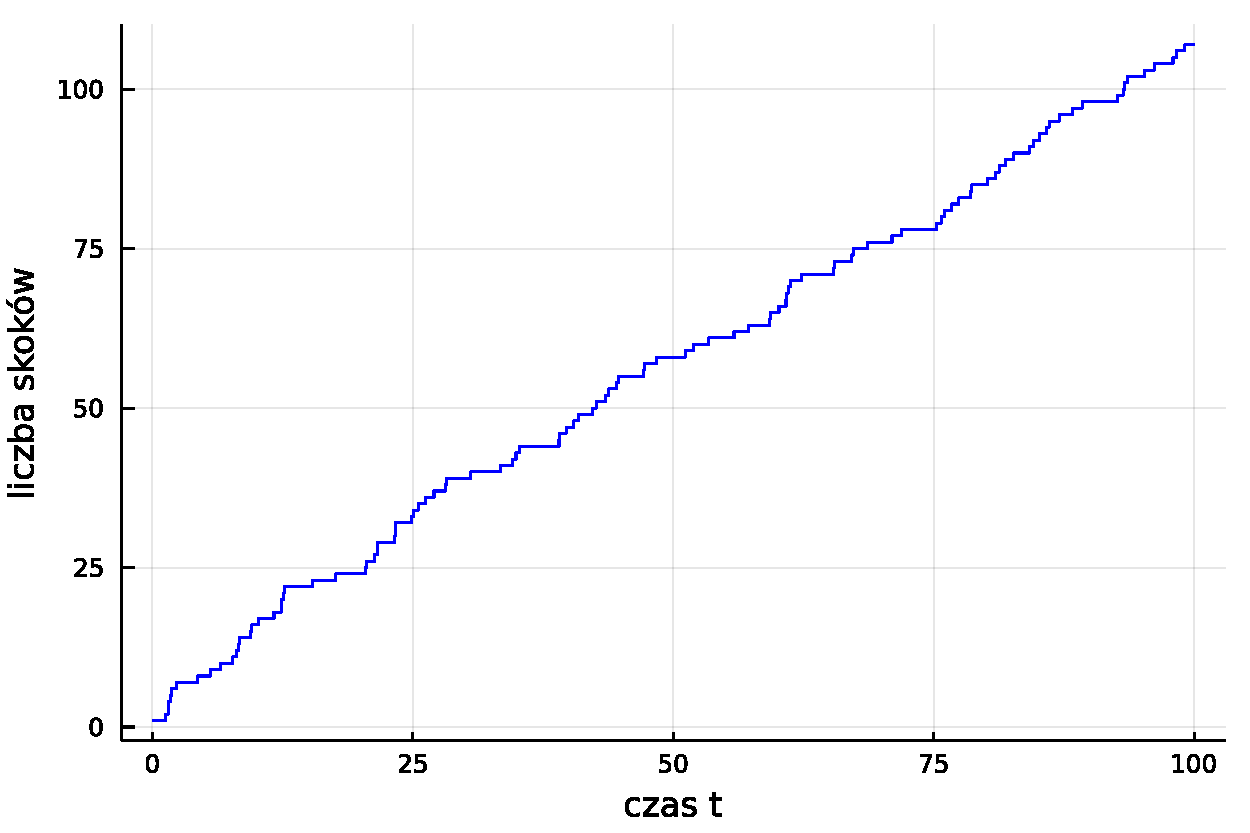
\includegraphics[scale=0.35]{trajektoria_poissona.pdf}
	\caption{Przykładowa trajektoria procesu Poissona}
	\label{fig: 1}
\end{figure}

Aby wysymulować pojedynczą trajektorię procesu Poissona, wykorzystamy fakt, że czasy oczekiwania na kolejny skok pochodzą z rozkładu wykładniczego o parametrze $\lambda$. \eqref{eq: 1.13}
Jeśli znamy wektor kolejnych skoków $N(t)$, to wiemy też, jak wygląda cała trajektoria $N(t)$. Przykład możemy zobaczyć na rys. \ref{fig: 1}.\\

Niech $T$ będzie oznaczać czas oczekiwania na kolejny skok w Jednorodnym Procesie Poissona z parametrem intensywności $\lambda$.
\begin{equation}
P(T>\tau) = P(N(\tau)=0) = \e^{-\lambda t} \Rightarrow T \sim Exp(\lambda) \label{eq: 1.13}.
\end{equation}

Algorytm:

\begin{enumerate}
\item Wstaw $I=0$, $t =0$.
\item Generuj $U\sim U(0,1)$.
\item Wstaw $t = t - \frac{\log{U}}{\lambda}$. Jeśli $t>T$ STOP. W przeciwnym razie wstaw $I = I+1$, $S_I=t$.
\item Wróć do 2.
\end{enumerate} 

Sprawdźmy poprawność tego algorytmu. Narysujmy na wykresie (rys. \ref{fig: 2}) 100 trajektorii i nanieśmy średnią wartość procesu. Korzystając z definicji Jednorodnego Procesu Poissona wiemy, że w danym punkcie $t$, średnio powinniśmy znaleźć się w punkcie $\lambda t$.
Rzeczywiście, trajektorie oplatają wartość średnią. Na tej podstawie stwierdzamy, że generator trajketorii jest poprawny.

\begin{figure}[H]
	\center
	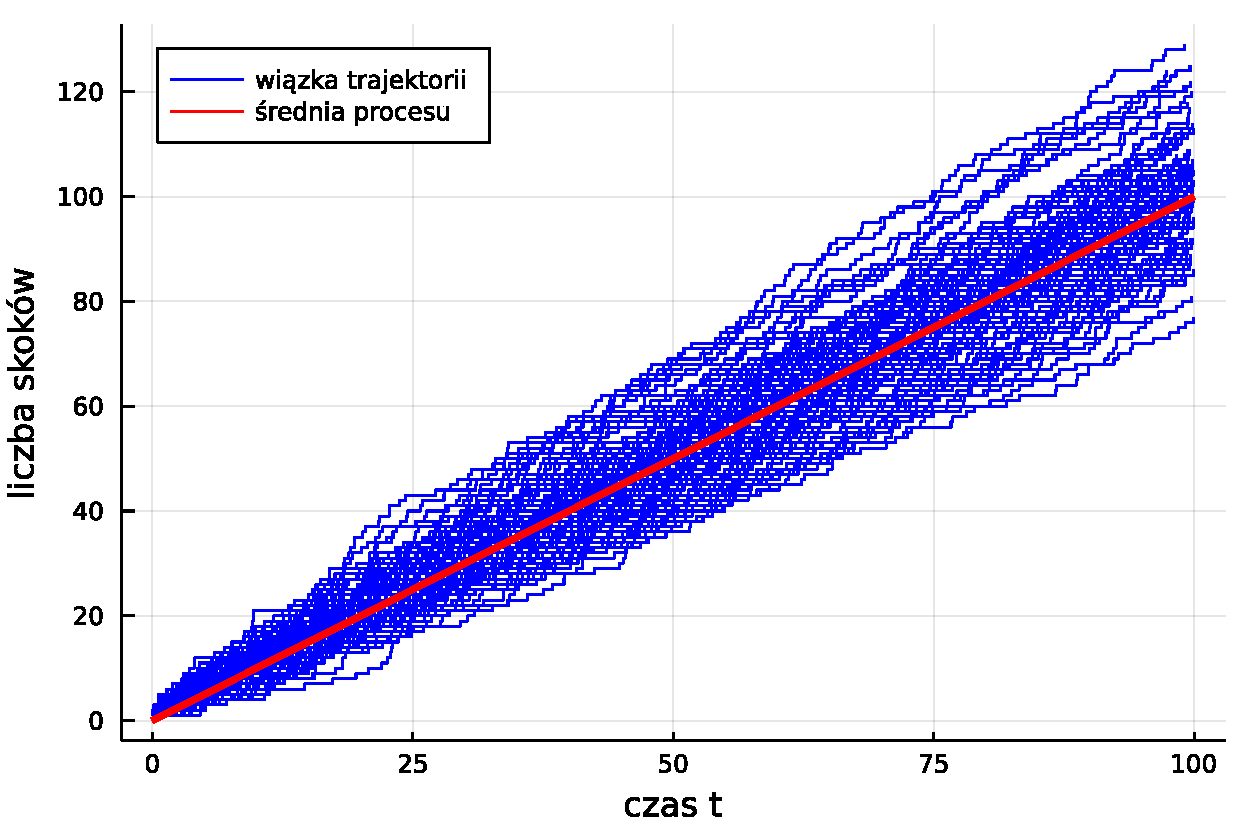
\includegraphics[scale=0.35]{poprawność_poissona.pdf}
	\caption{Sprawdzenie poprawności algorytmu symulacji JPP}
	\label{fig: 2}
\end{figure}

\subsection{Proces Ryzyka}
\subsubsection*{Ogólny proces Ryzyka}

\textbf{Procesem Ryzyka} nazywamy proces stochastyczny opisujący kapitał firmy ubezpieczeniowej. Proces ten zadany jest wzorem $$R(t) = u + c(t) - \sum_{i=1}^{N(t)}X_i,$$
gdzie:
\begin{itemize}
\item $u>0$ - kapitał początkowy,
\item $c(t)$ - premia (przychody ze sprzedaży polis),
\item $N(t)$ - proces liczący straty,
\item $X_i$ - zmienna losowa $i.i.d.$, $X_i>0$, reprezentatywna wartość wypłaconych odszkodowań.
\end{itemize}

Oczywiście $c(t)$ powinno być dobrane w taki sposób, aby firma nie tylko nie zbankrutowała, ale także przynosiła zyski. W naszych rozważaniach przyjmujemy, że firma nie ma możliwości wzięcia kredytu. To znaczy moment, w którym kapitał firmy spada poniżej zera nazywamy \textbf{momentem~ruiny}.
Matematycznie: $$\tau(u) \buildrel def \over = \inf\{t\ge 0: R(t) < 0\}$$.\\
Zakładamy, że trajektorie procesu są lewostronnie ciągłe.
Zapiszmy algorytm pozwalając wykonać symulację $R(t)$ na zadanym przedziale czasowym $[0, T]$, $T>0$.\\
Algorytm:
\begin{enumerate}
\item Generuj $N(t)$ na $[0, T]$.
\item Generuj $X_1$, $X_2$, ..., $X_{N{T}}$.
\item Wstaw $R(t) = u + c(t) - \sum_{i=1}^{N(t)}X_i$.
\end{enumerate}
\subsubsection*{Klasyczny Proces Ryzyka}
W \textbf{Klasycznym Procesie Ryzyka} premia $c(t)$ jest funkcją liniową postaci $ct$, gdzie $c$ jest pewną stałą, natomiast $N(t)$ to Jednorodny Proces Poissona z intensywnością $\lambda > 0$. Aby wyznaczyć $c$, najpierw znajdźmy średnią stratę kapitału firmy ubezpieczeniowej:

\begin{equation}
\EX(\sum_{i=1}^{N(t)}X_i = \EX(\EX(\sum_{i=1}^{N(t)}X_i | N(t)) = \EX(\mu N(t)) = \mu \lambda t,
\end{equation}
gdzie $\mu$ - średnia wypłata odszkodowania ($\EX X_1$).\\
Więc już wiemy, że $c(t) >  \mu \lambda t$, ponieważ zakład chce zarobić. Aby dokładniej opisać naszą funkcję premii, wprowadźmy pojęcie \emph{narzutu} $\theta >0$, które będziemy interpretować jako tempo sprzedaży polis ubezpieczoniowych. Zapiszmy ostatecznie:

\begin{equation}
c(t) = (1+\theta)\mu \lambda t.
\end{equation}

Możemy już przedstawić pełną postać klasycznego procesu $R(t)$:

\begin{equation}
R(t) = u +  (1+\theta)\mu \lambda t- \sum_{i=1}^{N(t)}X_i.
\end{equation}

Przykładową trajektorię takiego procesu można zobaczyć na rys. \ref{fig: 3}.
 
\begin{figure}
	\center
	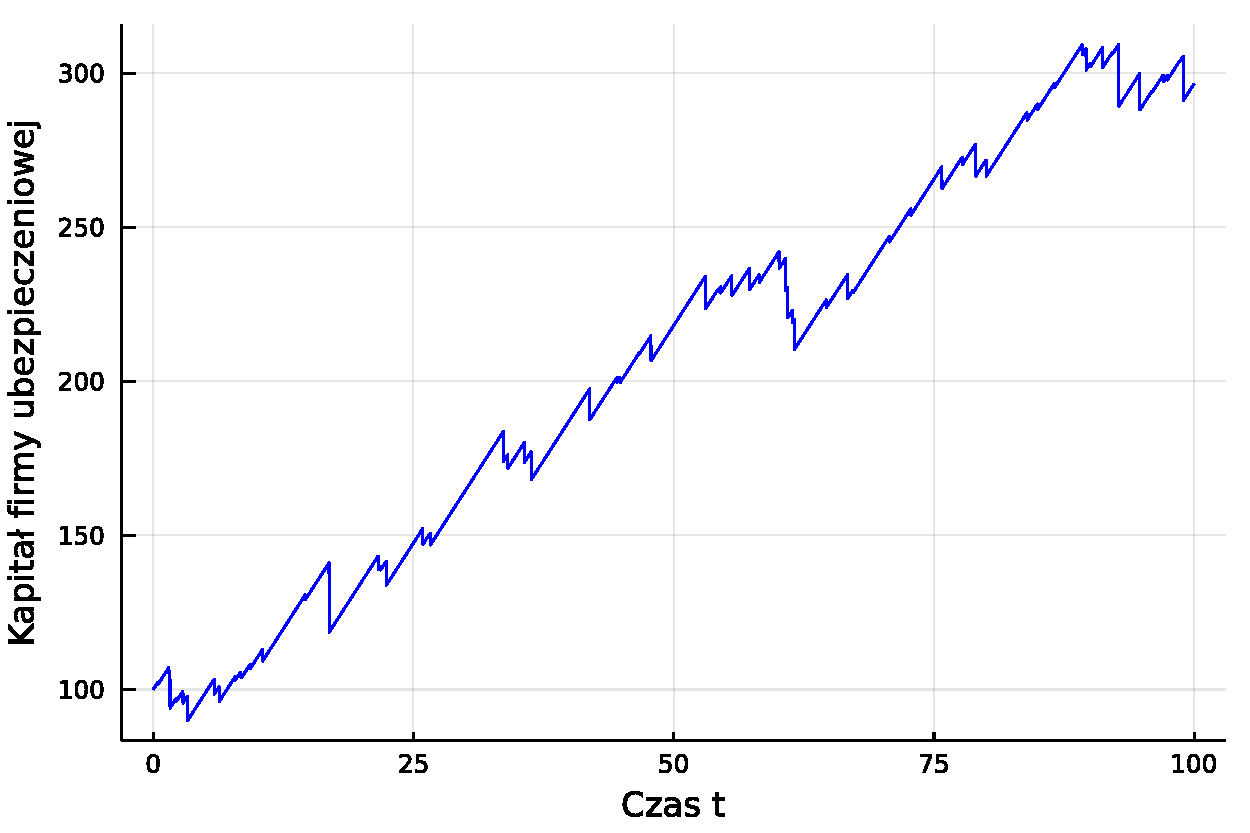
\includegraphics[scale=0.35]{trajektoria_ryzyka.pdf}
	\caption{Przykładowa trajektoria procesu Ryzyka}
	\label{fig: 3}
\end{figure}

\subsection{Ruch Browna}

\textbf{Ruchem Browna} (procesem Wienera) nazywamy proces stochastyczny $B = (B_t)_{t\geq0}$, taki że:
\begin{itemize}
	\item $B_0=0$.
	\item $B$ ma niezależne przyrosty.
	\item $B_t-B_s\sim N(0,~t-s)$, dla $0\leq s<t$.
	\item $B$ ma trajektorie ciągłe z prawdopodobieństwem 1.
\end{itemize}
W zadaniu będziemy posługiwać się jego zmodyfikowaną wersją:
$$B_t^x=B_t^0+x,$$
Gdzie $B_t^0$ to klasyczny ruch Browna. Oznacza to tyle, że proces $B_t^x$ rozpoczyna się w punkcie $x$. Chcąc uzyskać jego numeryczne przybliżenie przy pomocy symulacji komputerowej, wykorzystamy następujący algorytm:
\\ \\
Algorytm(0)
\begin{enumerate}
	\item $B_0^x=x$
	\item $B_{i+1}^x=B_{i}^x+dt^{\frac{1}{2}}\psi_i$
\end{enumerate}
gdzie $\psi_i\sim N(0,1),\quad i.i.d$, natomiast $dt$ to najmniejszy krok czasowy.\\ \\ 

Funkcja autokowariancji
\begin{gather}
	Cov(B_t,B_s)=\mathbb{E}(B_sB_t)-\mathbb{E}B_s\mathbb{E}B_t=\\
	=\mathbb{E}(B_s(B_sB_t))+\mathbb{E}(B_s^2)\\
	=\mathbb{E}B_s\mathbb{E}(B_sB_t)+\mathbb{E}B_s^2=s
\end{gather}
Ogólnie
$$Cov(B_t,B_s)=\min\{s,t\}$$

\begin{figure}[H]
	\center
	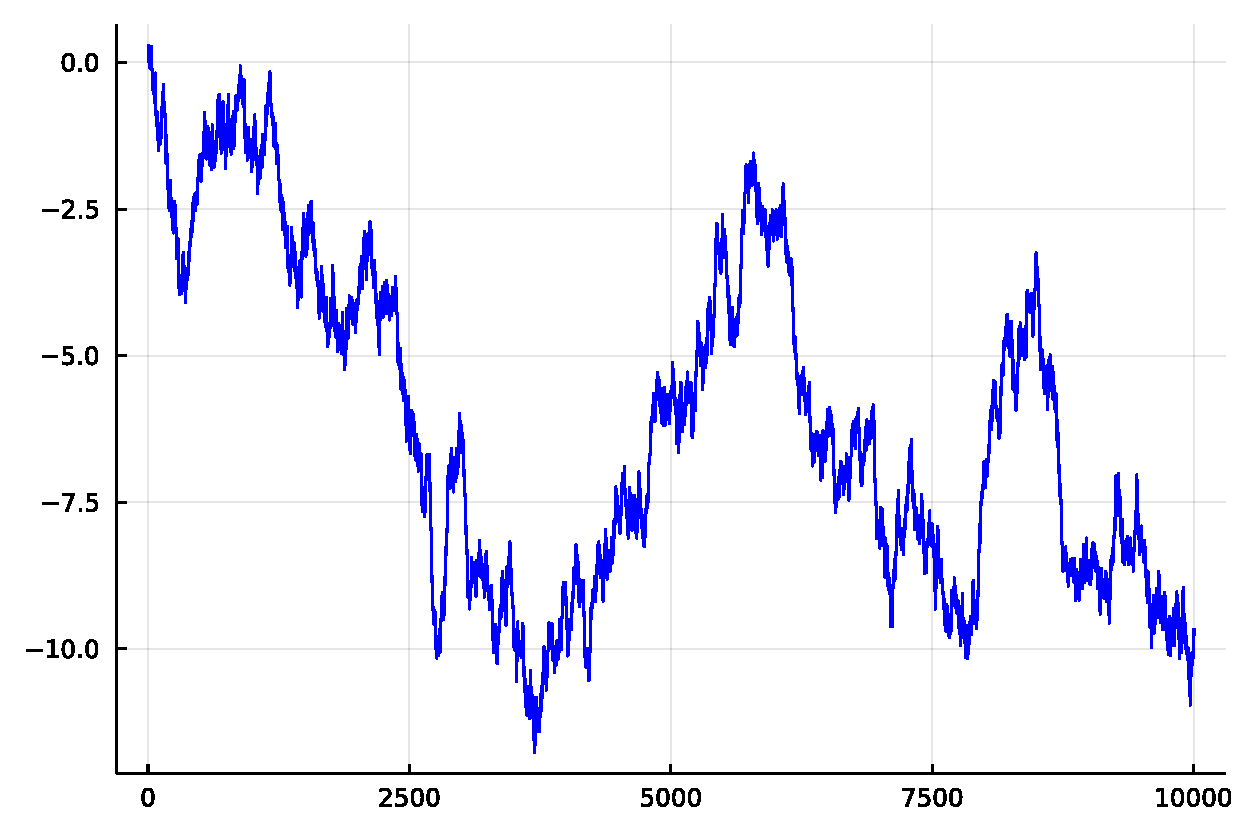
\includegraphics[scale=0.35]{przyklad_trajektorii.pdf}
	\caption{Przykładowa trajektoria Ruchu Browna}
	\label{fig: pojedyncza_browna}
\end{figure}

\begin{figure}[H]
	\center
	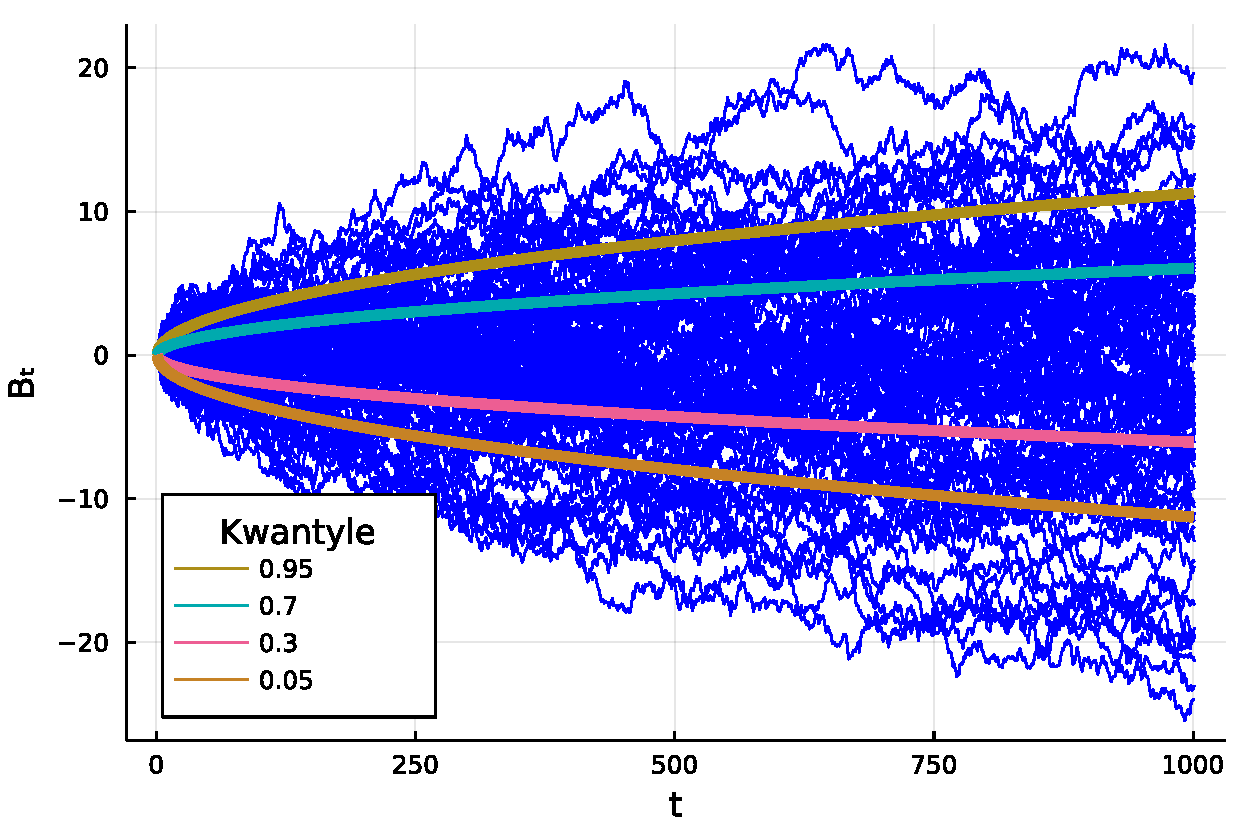
\includegraphics[scale=0.35]{kwantyle.pdf}
	\caption{Teoretyczne kwantyle na tle stu trajektorii}
	\label{fig: wiązka_browna}
\end{figure}



\section{Analiza wybranego klasycznego modelu procesu Ryzyka}


\subsection{Wizualizacja danych}

Dysponujemy 50-cioma trajektoriami z pewnego klasycznego procesu Ryzyka $R(t)$ wygenerowanych na odcinku $[0,T]$, $T= 100$ z krokiem $h = 0.01$ i kapitałem początkowym $u=50$. Naszym pierwszym celem będzie znalezienie jawnej postaci $R(t)$.\\
Zacznijmy od zwizualizowania danych trajektorii na wykresie \ref{fig: wizualizacja}. Niestety, z samego wykresu nie jesteśmy zbyt wiele wywnioskować. Z trajektorii odstających wnioskujemy, że rzeczywiście przyrost kapitału jest liniowy. Na ten moment nie wiemy nic o rozkładzie wypłat.
Widzimy za to kilka odstających trajektorii, które mogą zaniżać średnią wartość procesu.

\begin{figure}[H]
	\center
	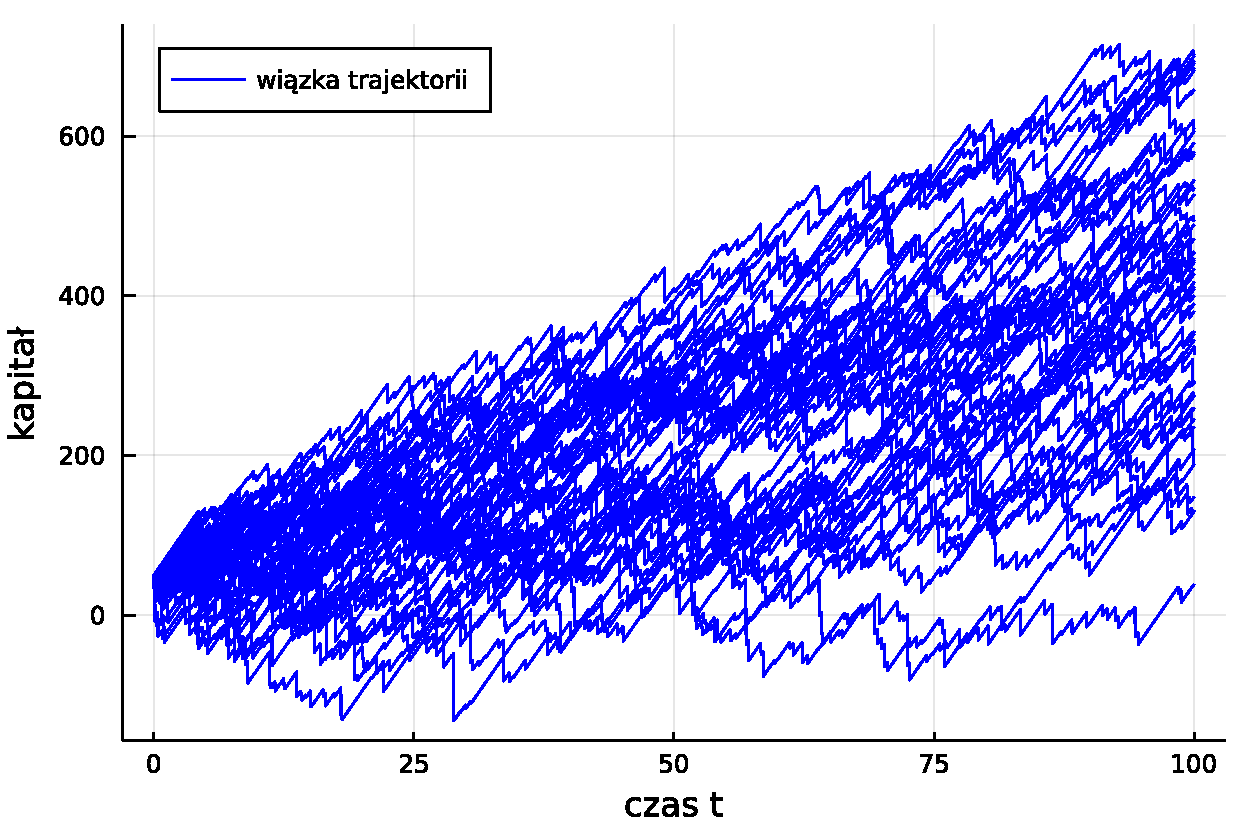
\includegraphics[scale=0.35]{wizualizacja_trajektorii.pdf}
	\caption{Przykładowa trajektoria procesu Ryzyka}
	\label{fig: wizualizacja}
\end{figure}

\subsection{Oszacowanie parametru intensywności procesu Poissona}

Pomysł: Jeśli $N(t)$ to jednorododny proces Poissona z parametrem intensywności $\lambda$, to czasy oczekiwania na kolejny skok są z rozkładu wykładniczego z tym samym parametrem, co już pokazaliśmy wcześniej. W związku z tym należy znaleźć momenty tych skoków, a następnie z nich wyłuskać czasy oczekiwania pomiędzy kolejnymi skokami. Otrzymamy prostą próbę losową z rozkładu wykładniczego z parametrem $\lambda$.
Następnie, za pomocą metody momentów oraz największej wiarogodności wyestymujemy porządany parametr.

\subsubsection*{Wektor momentów skoków}

Trajektoria to pewien wektor przedstawiający kapitał firmy ubezpieczeniowej w pewnym czasie $\tau$. Oczywiście do momentu wypłaty odszkodowania musi być ona rosnąca. Tym faktem posłużymy się znajdując momenty skoków.

Zapiszmy algorytm, który zapisze czasy $\tau^*$, w których nastąpił jakikolwiek spadek w kapitale. Zakładamy przy tym, że trajektoria jest lewostronnie ciągła.

\begin{enumerate}
\item Ustal $\tau=0$, $h=0.01$, $I = 1$, trajektorię ryzyka $R$ oraz pusty wektor $V.$
\item. Zwiększ czas $\tau$ o krok $h$, zwiększ $I$ o jeden.
\item. Sprawdź, czy firma odnotowała spadek ($R[I] < R[I-1]$). Jeśli tak, wstaw $\tau$ do wektora $V$. W przeciwnym przypadku kontynuuj.
\item. Powtarzaj 2-3, dopóki $I < \#R$.
\item Zwróć $V.$
\end{enumerate}

\subsubsection*{Wektor czasów oczekiwania}

Mając do dyspozycji momenty skoków, w bardzo łatwy sposób jesteśmy w stanie znaleźć czasy ocekiwania. Weźmiemy po prostu różnice kolejnych momentów. Powtórzymy cały proces dla każdej z trajektorii, a następnie złączymy wszystkie wektory w jeden. Możemy tak zrobić, gdyż każda symulacja jest od siebie nie zależna. Zwiększymy przy tym dokladność estymatorów.

Algorytm:

\begin{enumerate}
\item Znajdź wektor momentów skoków $V$.
\item Ustal liczność $k$ wektora $V$.
\item Stwórz wektor czasów oczekiwania $T_j$ o długości $k-1$.
\item Ustal $T[1] = V[1]$, $I=2$
\item Wstaw $T[I] = V[I] - V[I-1]$.
\item Zwiększ $I$ o jeden.
\item Powtórz kroki 5-6 $k-2$ razy.
\item powtórz kroki 1-7 dla każdej z trajektorii
\item Wstaw $T = \bigcup T_j$.
\end{enumerate}

W naszym przypadku $j = 1, 2, ...,50$. Dla formalności przedstawmy otrzymany wektor na histogramie częstości. Upewniamy się w ten sposób, że nie popełniliśmy błędu.
Przypomnijmy, że nasz wektor czasów oczekiwania jest dosyć dużą próbą losową z rozkładu wykladniczego z parametrem $\lambda$. Do estymacji tego parametru posłużymy się metodami największej wiarogodności oraz momentów.

METODA NAJWIĘKSZEJ WIAROGODNOŚCI

METODA MOMENTÓW

Okazuje się, że te dwa estymatory są sobie równe. Z teorii statystyki wiemy również, że są asymptotycznie nieobciążone. Po podstawieniu do wzoru otrzymujemy, że nasze $$\lambda = 1.4681753373312858.$$ Celowo nie zaokrąglamy wartości, by jak najdokładniej odzwierciedlić analizowany proces.

\begin{figure}[H]
	\center
	\includegraphics[scale=0.35]{histogram_czasów.pdf}
	\caption{Histogram częstości czasów oczekiwania na kolejny skok}
	\label{fig: 4}
\end{figure}

\subsection{Znalezienie rozkładu wypłat odszkodowań}

Pomysł: Postąpimy podobnie jak w przypadku szacowania parametru intensywności procesu Poissona. W tym celu przeiterujemy się po całej trajektorii i ponownie znajdziemy miejsca, w których nastąpił skok.  Tym razem zapiszemy jednak różnicę w wartości kapitału firmy, a nie momenty skoków.

Algorytm:

\begin{enumerate}
\item Ustal $I = 1$, trajektorię ryzyka $R$ oraz pusty wektor $X_j.$
\item Zwiększ $I$ o jeden.
\item Wyznacz $\Delta R = R[I-1] - R[I]$.
\item Jeśli $\Delta R >= 0$, wstaw wynik do wektora $V$.
\item. Powtarzaj 2-3, dopóki $I < \#R$.
\item. Zwróć $X.$
\item Powtórz kroki 1-6 dla każdej z trajektorii.
\item Wstaw $X = \bigcup X_j$.
\end{enumerate}

Ponownie otrzymujemy próbę losową. Tym razem nie znamy jednak jej rozkładu. Rozkład częstości pokazany na histogramie bardzo przypomina rozkład wykładniczy. W związku z tym użyjemy testów statystycznych omówionych w poprzednim dziale, by sprawdzić, czy nasza próba może pochodzić z rozkładu właśnie wykładniczego.  Wyznaczymy p-wartość testów. Jeśli przekroczą one wartości 0.05 w obu przypadkach, przyjmiemy hipotezę zerową na poziomie istotności 5\%. Wyniki gromadzimy w tabeli (ODWOŁAĆ SIĘ) i odczytujemy, że rzeczywiście dane mogą pochodzić z rozkładu wykładniczego. Po porównaniu dystrybuant teoretycznej i empirycznej nie mamy już wątpliwości. Dysponujemy próbą losową z rozkładu wykładniczego!
Pozostaje wyestymować jej parametr $\rho$. Podstawiając do wzoru (ODWOŁAĆ SIĘ) otrzymujemy, że

\begin{equation}
 	\rho = 0.09901122812369685.
\end{equation} 

\begin{figure}[H]
	\center
	\includegraphics[scale=0.35]{histogram_wypłat.pdf}
	\caption{Histogram częstości wartości wypłat odszkodowań}
	\label{fig: 5}
\end{figure}

\subsection{Obliczenie wartości parametru narzutu}

Premię wyznaczymy na dwa sposoby. Najpierw bardziej uniwersalnym, działającym nie tylko w przypadku klasycznego procesu ryzyka, a potem korzystając właśnie z tego faktu. \\
Najpierw spójrzmy na wzór (ODWOŁAĆ SIĘ - $R(t)$). Po krótkim zastanowieniu dochodzimy do wniosku, że średnio nasz proces powinien wzrastać o $\theta \frac{1}{\rho} \lambda$ (POKAZAĆ).
Wyznaczymy więc empiryczną średnią wartość procesu z naszego zestawu trajektorii, a następnie wyznaczymy metodą regresji liniowej, korzystając z \emph{np. polyfit}, prostą, której współczynnik kierunkowy powinien być równy naszej teoretycznej średniej procesu.
Znając $\rho$ oraz$ \lambda$, podstawimy do wzoru i otrzymamy nasz pożądany parametr.

ALGORYTM

Ostatecznie otrzymujemy, że $$\theta = 0.2526239274374162$$.


\subsection{Sprawdzenie poprawności wyników}

Mając do dyspozycji jawną postać naszego procesu ryzyka możemy generować nowe trajektorie. Na rysunku \ref{fig: 7} zamieszczamy nowych trajektorii. Nałożymy na nim jedną losowo wybraną trajektorię z zestawu danych. Zaznaczymy również średnią empiryczną z zestawu danych.
Na rysunku \ref{fig:8} porównujemy średnią empiryczną z 50-ciu nowych trajektorii z teoretyczną, na tle empirycznej z zestawu danych. Na \ref{fig:9} robimy to samo, tylko zwiększamy liczbę nowych trajektorii do $N=1000$. Widzimy, że dla większej liczby trajektorii, średnia empiryczna niemal nie odrywa się od teoretycznej.
Natomiast dla małej próby, tak jak w zestawie danych, mogą nastąpić mniej lub bardziej poważne odchylenia. Możemy otrzymać nawet bardziej ekstremalne przypadki. Wystarczy dostatecznie długo generować małą wiązkę trajektorii. W końcu natrafimy na osobliwy przypadek.

\begin{figure}[H]
	\center
	\includegraphics[scale=0.35]{100_trajektorii_ryzyka.pdf}
	\caption{Przykładowa wiązku stu trajektorii procesu ryzyka dla naszych parametrów}
	\label{fig: 7}
\end{figure}

\begin{figure}[H]
	\center
	\includegraphics[scale=0.35]{porównanie_średnich_procesu_ryzyka.pdf}
	\caption{Porównanie średnich empirycznych}
	\label{fig: 8}
\end{figure}

\subsection{Prawdopodobieństwa bankructwa}

\subsubsection{W czasie skończonym}

\textbf{prawdopodobieństwo ruiny w skończonym czasie} definiujemy jako
\begin{equation}
\psi(u,T)=P(\tau(u)<T),
\end{equation}
gdzie:
\begin{itemize}
\item $u > 0$ - kapitał początkowy,
\item $T > 0$ - badany okres.
\end{itemize}

Najczęściej $\psi(u,T)$ musimy wyznaczać symulacyjnie. Jednak w przypadku, gdy zmienne losowe odpowiadające za wypłaty są z rozkładu wykładniczego, znamy jego teoretyczną wartość. Zapiszmy jego postać dla przypadku, gdy $c=1$, $\rho = 1$. \\
Tutaj $c$ - premia, $\rho$ - parametr rozkładu wykładniczego.

Mamy wtedy:

\begin{equation}
\psi(u,T)=\lambda \exp(-(1-\lambda)u)-\frac{1}{\pi} \int\limits_{0}^{\pi}\frac{f_1(x)f_2(x)}{f_3(x)}\diff{x}, \label{eq:ruina_teoretyczna}
\end{equation}
gdzie:
$$f_1(x)=\lambda \exp(2\sqrt{\lambda}T\cos x - (1+\lambda)T + u(\sqrt{\lambda}\cos x -1)),$$
$$f_2(x)=\cos(u\sqrt{\lambda}\sin x) - \cos(u\sqrt{\lambda}\sin x +2x),$$
$$f_3(x) = 1+\lambda - 2\sqrt{\lambda}\cos x.$$
Dla $\rho\ne1$ korzystamy z faktu, że prawdopodobieństwo ruiny
$$\psi_{\lambda,\rho}(u,T)=\psi_{\frac{\lambda}{\rho},1}(\rho u,\rho T).$$
Dla $c\ne 1$ korzystamy z faktu, że
$$\psi_{\lambda,c}(u,T)=\psi_{\frac{\lambda}{c},1}(u,cT).$$

Trzeba jednak przyznać, że korzystanie z \eqref{eq:ruina_teoretyczna} może być mało praktycznie, a zwykle - po prostu niemożlwe. Zamiast tego możemy wygenerować $N$ trajektorii i zliczać te, które spadły poniżej zera. Wydaje się to o wiele prostsze.\\

Algorytm\\
\begin{enumerate}
	\item Generuj N trajektorii $R^{(1)}(t),\dots,R^{(N)}(t)$ procesu ryzyka na [0,T].
	\item Wyznacz $n=\#\{i\in\{1,\dots,N\}:\min_{T\in[0,T]}R^{(i)}(t)<0\}$.
	\item Wstaw $\psi(u,T)=\frac{n}{N}$.
\end{enumerate}

Nasze wyniki umieszczamy w tabeli (ODWOŁAĆ SIĘ)

\subsubsection{W czasie nieskończonym}

\textbf{Prawdopodobieństwo ruiny w nieskończonym czasie} definiujemy jako\\

\begin{equation}
\psi(u)=P(\tau(u)<\infty),
\end{equation}

gdzie $u > 0$ - kapitał początkowy. \\
\\
Wyznaczenie tego prawdopodobieństwa może wydawać się trudne. Mamy bowiem do czynienia z czasem nieskończonym, a to.. dosyć długo. Na szczęście matematykom udało się rozwiązać ten problem.
Sukces ten przypisuje się dwóm wybitnym matematykom - F. Pollaczkowi oraz A.Chinczynowi. Ich wynik zapisujemy w \eqref{eq: polchin}.
\\\\
\begin{equation}
\psi(u)=\frac{\theta}{1+\theta}\sum_{n=0}^{\infty}\left(\frac{1}{1+\theta}\right)^n\cdot B_n(u), \label{eq: polchin}
\end{equation}
gdzie $B_n(u)=P(Y_1+\dots+Y_n>u)$ oraz $Y_i$ to zmienne losowe \emph{i.i.d.} o gęstości $f(x)=\frac{1-F_{X_i}(x)}{\EX{X_i}}$.\\

W naszym przypadku wielkości wypłat są z rozkładu wykładniczego. W związku z tym postać $\psi(u)$ powinna być znana. Policzmy $\psi(u)$.
Mamy 
\begin{equation}
X_i\sim Exp(\rho) \Rightarrow f(x)=\frac{1-(1-e^{-\rho x})}{\frac{1}{\rho}}=\rho e^{-\rho x} \sim Exp(\rho).\\
\end{equation}

Skoro $Y_i$ jest z rozkładu wykladniczego, to suma wszystkich $Y_i$ będzie z rozkładu Erlanga (gamma z parametrami $n$, $\rho$). Ten fakt udowodniliśmy w poprzednim raporcie.
Podstawiając do \eqref{eq: polchin} i wstawiając wzór na gęstość rozkładu Erlanga:

\begin{gather}
	\psi(u)=\frac{\theta}{1+\theta}\sum_{n=1}^{\infty}\left(\frac{1}{1+\theta}\right)^n\int\limits_{u}^{\infty}\frac{(\rho x)^{n-1}}{(n-1)!} \rho e^{-\rho x}\diff{x} \\
	=\frac{\theta \rho}{(1+\theta)^2} \int\limits_{u}^{\infty}\rho e^{-\rho x}\sum_{n=1}^{\infty}\left(\frac{1}{1+\theta}\right)^{n-1}\frac{(\rho x)^{n-1}}{(n-1)!}\diff{x}\\
\end{gather}

Jeśli dobrze się przyjrzymy, to zauważymy, że suma pod całką jest tak na prawdę rozwinięciem Maclaurina funkcji $e^{\frac{\rho x}{1+\theta}}$. Podstawiając ją, otrzymujemy łatwą do przeliczenia całkę:

\begin{gather}
	=\frac{\theta\rho}{(1+\theta)^2}\int\limits_{u}^{\infty} e^{-\rho x} e^{\frac{\rho x}{1+\theta}}\diff{x}= \frac{\theta\rho}{(1+\theta)^2}\int\limits_{u}^{\infty} e^{-\rho (x-\frac{x}{1+\theta})}\diff{x}\\
	=\frac{\theta\rho}{(1+\theta)^2}\int\limits_{u}^{\infty} e^{-\rho (x\frac{\theta}{1+\theta})}\diff{x} = \frac{1}{1+\theta} e^{-\rho u \frac{\theta}{1+\theta}}.
\end{gather}

Więc ostatecznie zapisujemy \eqref{eq: teoretyczny_nieskończony}:

\begin{equation}
\psi(u) = \frac{1}{1+\theta} e^{-\rho u \frac{\theta}{1+\theta}}. \label{eq: teoretyczny_nieskończony}
\end{equation}

Metoda Monte Carlo dla $\psi(u)$\\ \\
Fakt
$$\psi(u)=P(Y_1+\dots+Y_K>u),\quad \mathrm{gdzie} K\sim Geom(\frac{\theta}{1+\theta}), \quad K\indep Y_i.$$
Dowód
\begin{gather}
	P(Y_1+\dots+Y_K>u)=\sum\limits_{n=0}^{\infty}P(Y_1+\dots+Y_n>u)P(K=n)\\= \sum\limits_{n=0}^{\infty}P(Y_1+\dots+Y_n>u)(\frac{\theta}{1+\theta})(\frac{1}{1+\theta})^{n}=\psi(u)
\end{gather}
Algorytm\\
For $i=1:N$
\begin{enumerate}
	\item Generuj $K\sim Geom(\frac{\theta}{1+\theta})$.
	\item Generuj $Y_1,\dots,Y_K$- i.i.d o gęstości  $f(x)=\frac{1-F_{X_i}(x)}{\mu}$.
	\item Jeśli $Y_1+\dots+Y_K>u$, wstaw $Z(i)=1$, w przeciwnym wypadku $Z(i)=0$
\end{enumerate}
end\\
Wstaw $\psi(u)=\frac{Z(1)+\dots+Z(N)}{N}$

\section{Wybrane zależności trajektorii procesu Wienera}

\subsection{Średni czas wyjścia z danego pzedziału}

Będziemy badać średni czas wyjścia z  przedziału $[a,b]$, dla $x\in[a,b]$. Oznaczmy go jako $$\mathbb{E}\tau_x \mathrm{,~gdzie~}\tau_x:=\inf\{t\geq0:B_t^x\notin(a,b)\}.$$ 
Ponieważ na komputerze nie jest możliwe wykonanie symulacji procesu Wienera w czasie ciągłym, ustalamy najmniejszy krok czasowy $dt$, potrzebny do zastosowania metody numerycznej. Aby móc jak najlepiej oszacować średni czas wyjścia, powtarzamy $n$ razy symulację dla danego~$x$.\\ \\
Algorytm(1):
\begin{enumerate}
	\item Ustal punkt startowy $x$, najmniejszy krok czasowy $dt$, liczbę powtórzeń symulacji $n$ oraz granice przedziału $a$ i $b$.
	\item Jeżeli $x=a$ lub $x=b$ zwróć 0.
	\item Ustal $T=0$ 
	\item Generuj trajektorię procesu Wienera $B_t^x$ dopóki $B_t^x\leq a$ lub $B_t^x\geq b$.
	\item Zwiększ $T$ o ilość kroków czsowych $dt$, które mineły do tego momentu.
	\item Powtórz kroki 4-5 $n$ razy.
	\item Zwróć $\frac{T}{n}$.
\end{enumerate}
Chcąc zbadać zależność średniego czasu wyjścia od odległości punktu startowego $x$ do granic przedziału $[a,b]$ musimy ustalić $dx$, czyli różnicę między kolejnymi początkowymi $x \in [a,b]$.\\ \\ 
Algorytm(2):
\begin{enumerate}
	\item Ustal różnicę $dx$, najmniejszy krok czasowy $dt$, liczbę powtórzeń symulacji $n$, oraz granice przedziału $a$ i $b$.
	\item Stwórz pusty wektor $y$.
	\item Stwórz wektor $v$, początkowych $x$-ów należących do przedziału $[a,b]$, tak aby $v[i+1]-v[i]=dx$.
	\item Dla każdego elementu z wektora $v$ oblicz średni czas wyjścia (Algorytm(1)) i wstaw otrzymany wynik do wektora~$y$.
	\item Zwróć $y$
\end{enumerate}
Mając powyższe informacje, możemy przeprowadzić symulację. Rozważmy przypadki dla $n=10^3$ i $n=10^5$, $dt=0.1$, $dx=1$, $a=50$, $b=150$. Otrzymujemy wyniki widoczne na rys. \ref{fig:a1} i rys. \ref{fig:a2}
\begin{figure}[H]
	\begin{multicols}{2}
	\begin{center}
	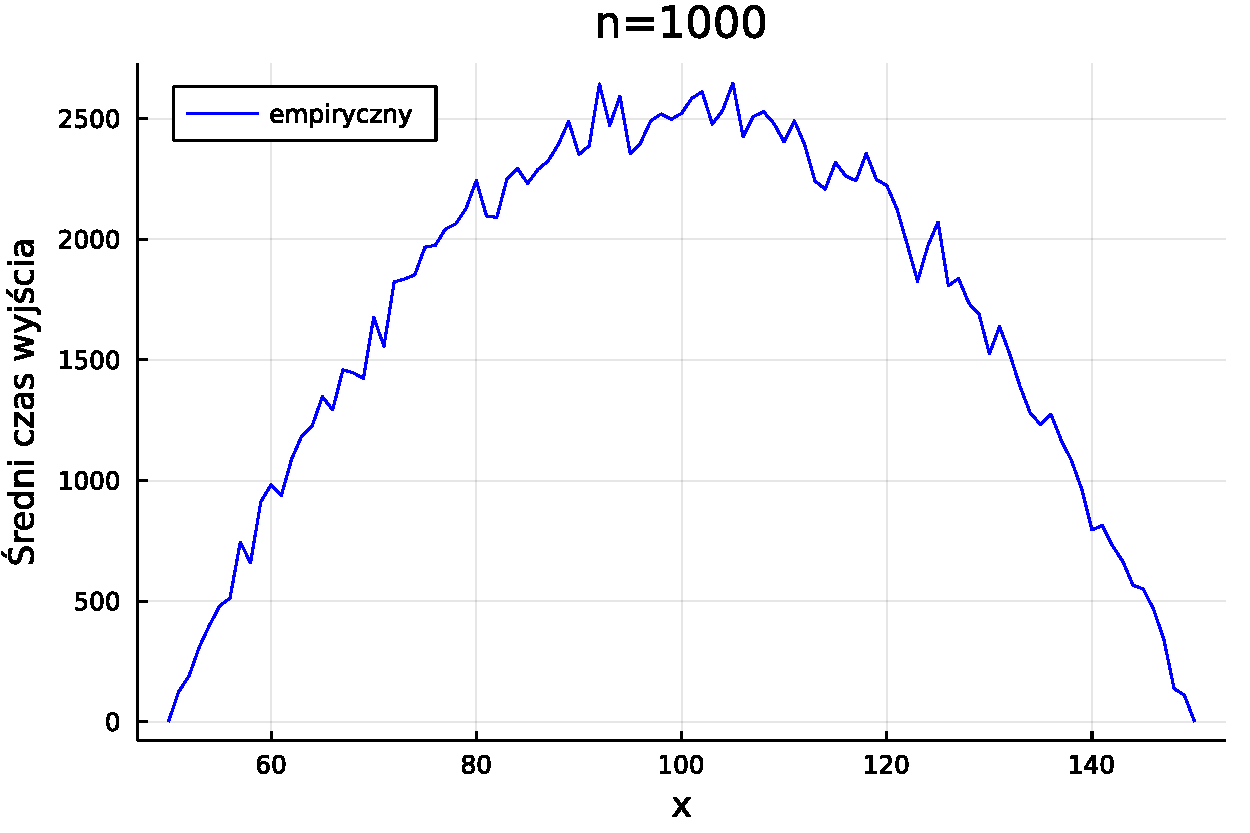
\includegraphics[scale=0.30]{time100.pdf}
	\caption{}
	\label{fig:a1}
	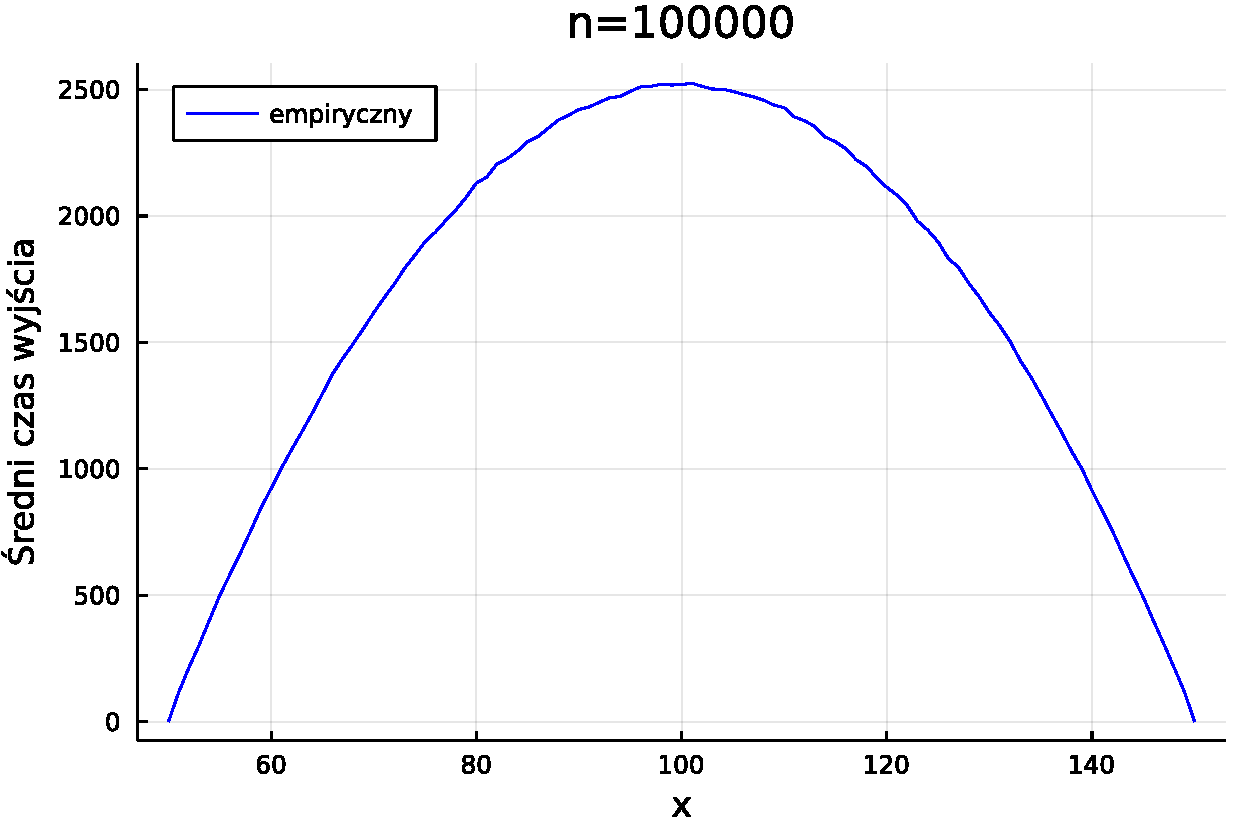
\includegraphics[scale=0.30]{time100000.pdf}
	\caption{}
	\label{fig:a2}
	\end{center}
	\end{multicols}
\end{figure}
Spróbujemy aproksymować funkcję, która opisuje otrzymane wyniki. Po kształcie wykresu przypuszczamy, że może to być wielomian co najmniej stopnia II na przedziale $[a,b]$. Wiemy również, że jego zera znajdują się w punktach $a$ oraz $b$, ponieważ czas wyjścia w przypadku gdy $x=a$ lub $x=b$, będzie wynosił 0. Załóżmy więc, że jest to funkcja kwadratowa, po zapisaniu w postaci kwadratowej wygląda następująco:
$$f(x)=\alpha(x-a)(x-b),$$
gdzie $\alpha$ jest szukanym współczynnikiem. W rozważanym przez nas przypadku:
$$f(x)=\alpha(x-50)(x-150).$$
Aby znaleźć współczynnik $\alpha$ użyjemy modułu \textit{numpy.polyfit} \cite{polyfit}. Dla przypadku z $n=10^3$ otrzymujemy $\alpha~=~1.012$, natomiast dla $n=10^5$, $\alpha=-1.001$. Na wykresie \ref{fig:a} widzimy jak współczynnik $\alpha$ zmienia się wraz ze wzrostem $n$. Możemy przypuścić, że $\lim\limits_{n\rightarrow\infty}c=-1$. Podobnie średnia ze stu powtórzeń algorytmu(2) dla $n=1000$ wraz z aproksymacją \textit{numpy.polyfit} wskazała, że $\alpha=1$. Ostatecznie otrzymujemy:
$$f(x)=-(x-50)(x-150).$$

Zestawienie funkcji empirycznej z teoretyczną znajduje się na rys. \ref{fig:33} oraz rys. \ref{fig:44}.
\begin{figure}
	\begin{center}
		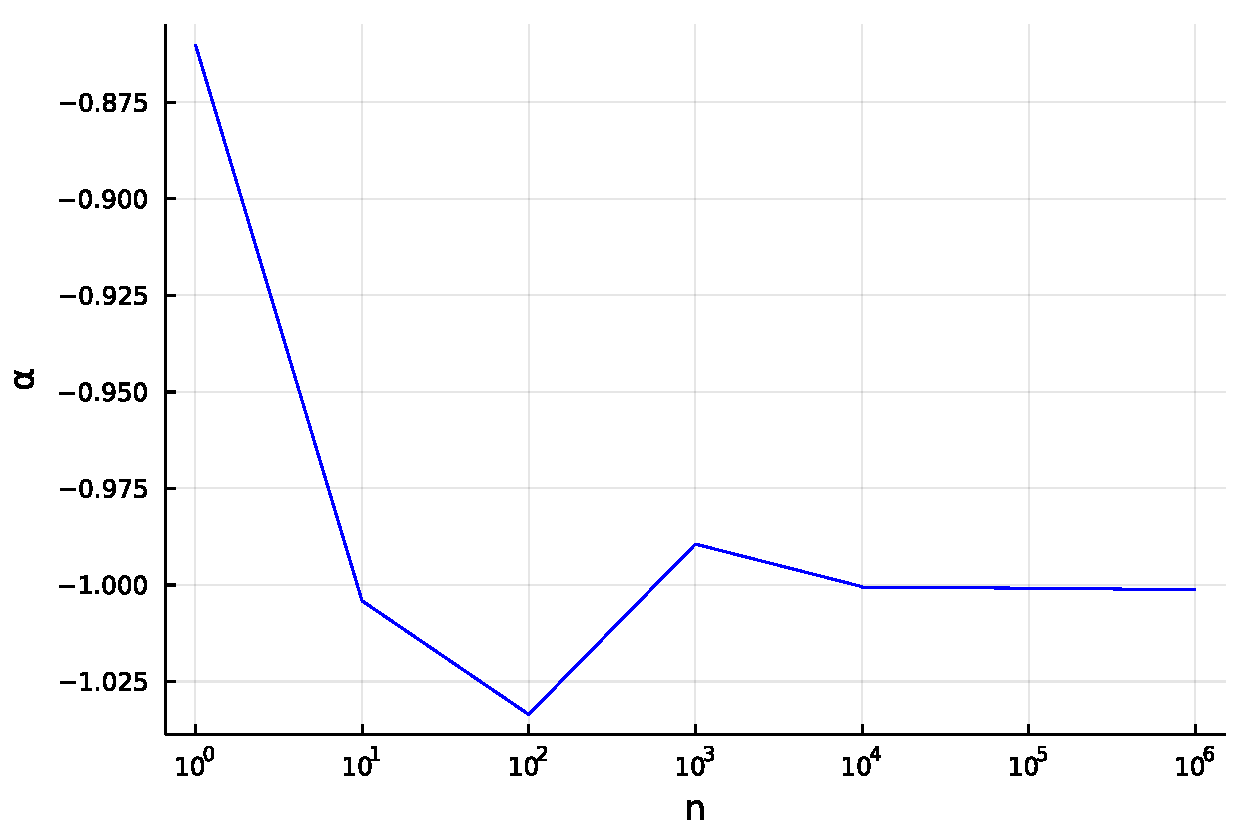
\includegraphics[scale=0.30]{alpha.pdf}
		\caption{}
		\label{fig:a}
	\end{center}
\end{figure}

\begin{figure}[H]
	\begin{multicols}{2}
		\begin{center}
			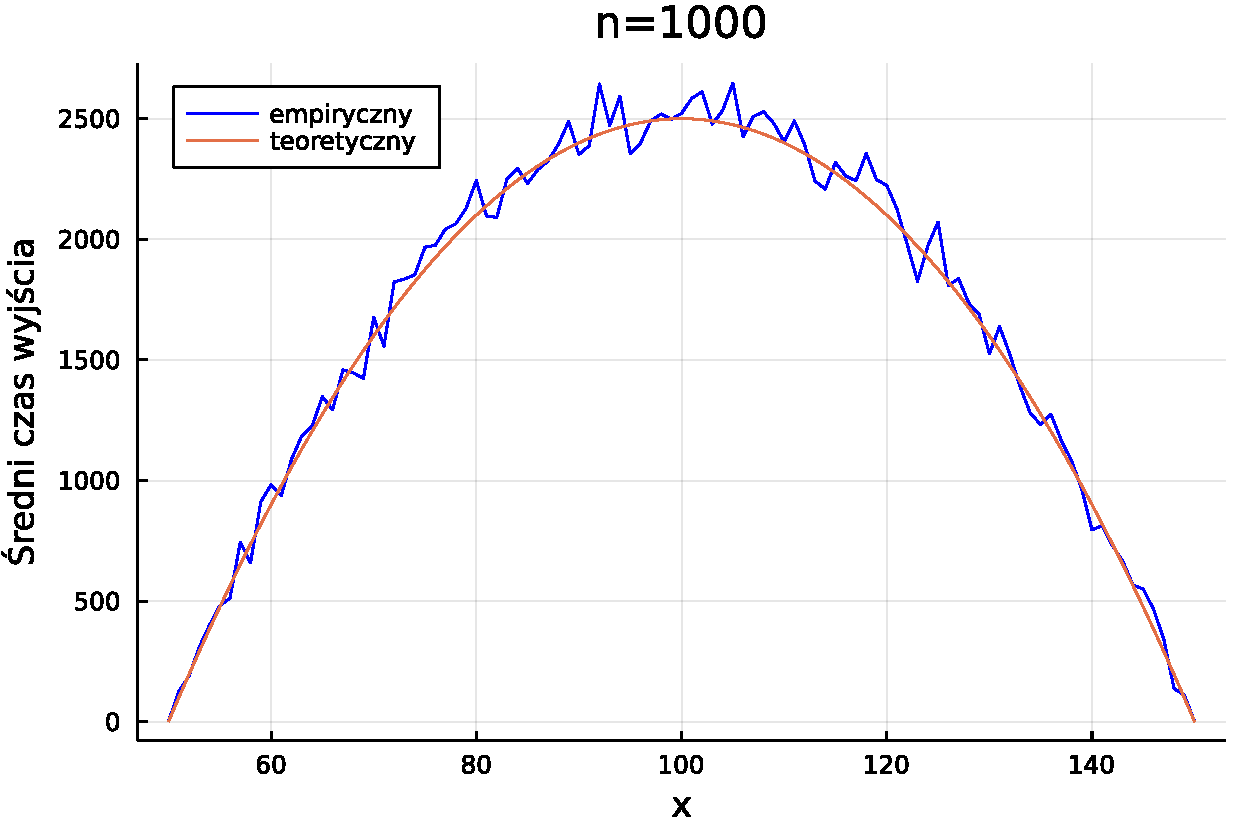
\includegraphics[scale=0.30]{time100poly.pdf}
			\caption{}
			\label{fig:33}
			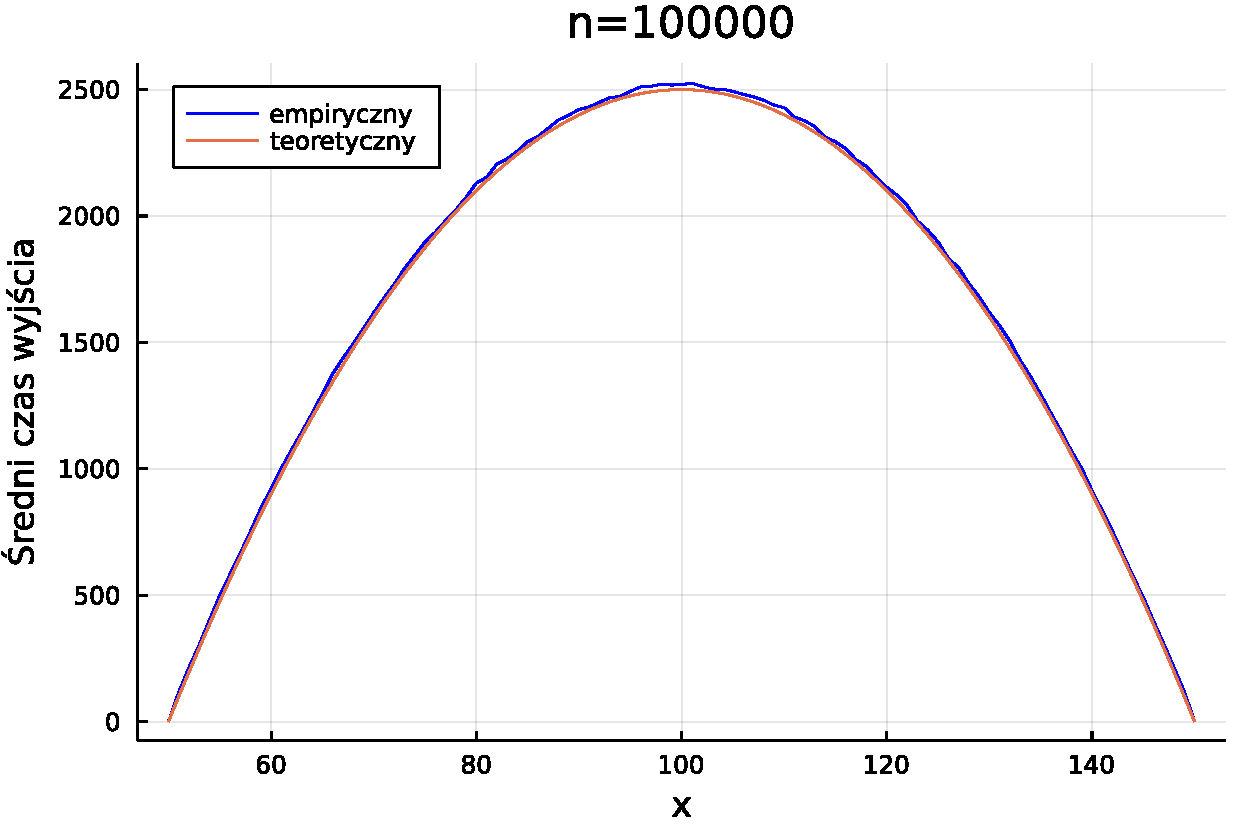
\includegraphics[scale=0.30]{time100000poly.pdf}
			\caption{}
			\label{fig:44}
		\end{center}
	\end{multicols}
\end{figure}

\subsection{Prawdopodobieństwo wyjścia przez wybraną granicę}

Przejdziemy teraz do szacowania, że wyjście nastąpiło przez granicę $b$, czyli:
$$P(B_{\tau^x}^x=b).$$
Jako, że symulacja działa w czasie dyskretnym, do określenia prawdopodobieństwa użyjemy wzoru:
$$P(B_{\tau^x}^x\geq b).$$
Postępujemy podobnie jak w przypadku szukania średniego czasu wyjścia.\\ \\
Algorytm(3):
\begin{enumerate}
	\item Ustal punkt startowy $x$, najmniejszy krok czasowy $dt$, liczbę powtórzeń symulacji $n$  oraz granice przedziału $a$ i $b$.
	\item Jeżeli $x=a$ zwróć 0.
	\item Jeżeli $x=b$ zwróć 1.
	\item Ustal $k=0$ 
	\item Generuj trajektorię procesu Wienera $B_t^x$ dopóki $B_t^x\leq a$ lub $B_t^x\geq b$.
	\item Jeśli $w\geq b$ zwiększ $k$ o jeden.
	\item Powtórz kroki 5-6 $n$ razy.
	\item Zwróć $\frac{k}{n}$.
\end{enumerate}
Analogicznie tworzymy algorytm, mający na celu zbadanie zależności między prawdopodobieństwem wyjścia przez $b$ a początkowym $x\in [a,b]$.\\ \\ 
Algorytm(4):
\begin{enumerate}
	\item Ustal różnicę $dx$, najmniejszy krok czasowy $dt$, liczbę powtórzeń symulacji $n$, oraz granice przedziału $a$ i $b$.
	\item Stwórz pusty wektor $y$.
	\item Stwórz wektor $v$, początkowych $x$-ów należących do przedziału $[a,b]$, tak aby $v[i+1]-v[i]=dx$.
	\item Dla każdego elementu z wektora $v$ oblicz prawdopodobieństwo wyjścia przez $b$ (Algorytm(3)) i wstaw otrzymany wynik do wektora~$y$.
	\item Zwróć $y$
\end{enumerate}
Korzystając z algorytmu 3 i 4, przeprowadzimy symulację dla $n=10^3$ i $n=10^5$, $dt=0.1$, $dx=1$, $a=50$, $b=150$. Otrzymujemy wyniki widoczne na rys. \ref{fig:55} i rys. \ref{fig:66}
\begin{figure}[H]
	\begin{multicols}{2}
		\begin{center}
			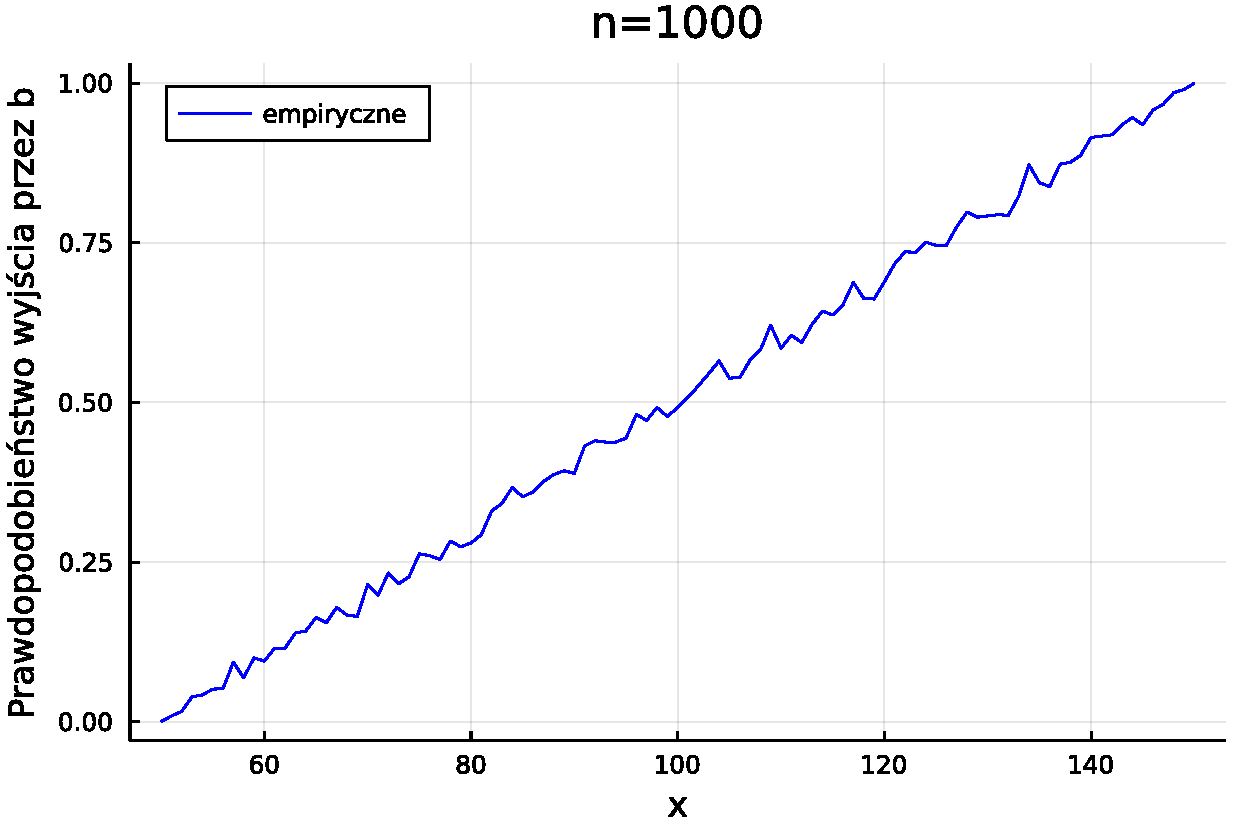
\includegraphics[scale=0.30]{prob100.pdf}
			\caption{}
			\label{fig:55}
			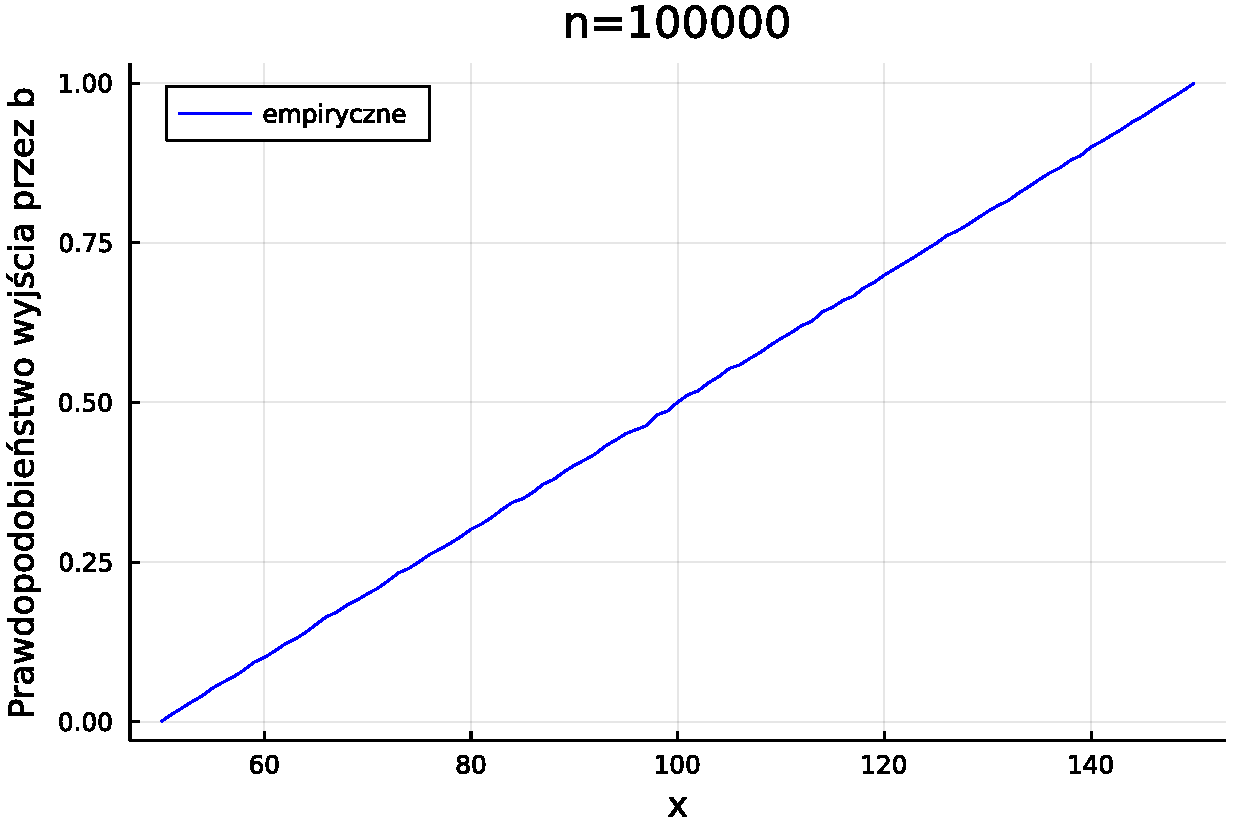
\includegraphics[scale=0.30]{prob100000.pdf}
			\caption{}
			\label{fig:66}
		\end{center}
	\end{multicols}
\end{figure}
Po kształcie wykresu spodziewamy się, że jest to funkcja liniowa. Kiedy początkowe $x=a$, prawdopodobieństwo wyjścia przez $b$ wynosi 0, natomiast gdy początkowe $x=b$, prawdopodobieństwo to będzie wynosić~1. Znając dwa punkty przez które przechodzi funkcja liniowa $f(x)=\beta x+\gamma$, gdzie $\beta$ i $\gamma$ są szukanymi parametrami, możemy wyprowadzić ogólny wzór rozwiązując następujący układ równań:
\[
\myarray{\beta a + \gamma = 0\\ \beta b + \gamma = 1}
\Leftrightarrow
\myarray{\beta = \frac{-1}{a-b} \\ \gamma = \frac{a}{a-b}}
\]
Zatem:
$$f(x)=-\frac{1}{a-b}x + \frac{a}{a-b}$$
Podstawiając nasze dane ($a=50$, $b=150$), otrzymujemy:
$$f(x)=\frac{1}{100}x-\frac{1}{2}$$
Sprawdzamy, czy moduł \textit{numpy.polyfit} da nam pdobny rezultat, przy jego pomocy otrzymujemy:
$$f(x)=0.00997x-0.497 \quad \mathrm{dla} \quad n=10^3$$
$$f(x)=0.01x-0.5 \quad \mathrm{dla} \quad n=10^5$$
Co zgadza się z naszymi teoretycznymi obliczeniami (im większe $n$ tym większa dokładność). Na wykresach zestawienie empirycznej i teoretycznej funkcji prezentuje się następująco (rys. \ref{fig:77} i rys. \ref{fig:88}):
\begin{figure}[H]
	\begin{multicols}{2}
		\begin{center}
			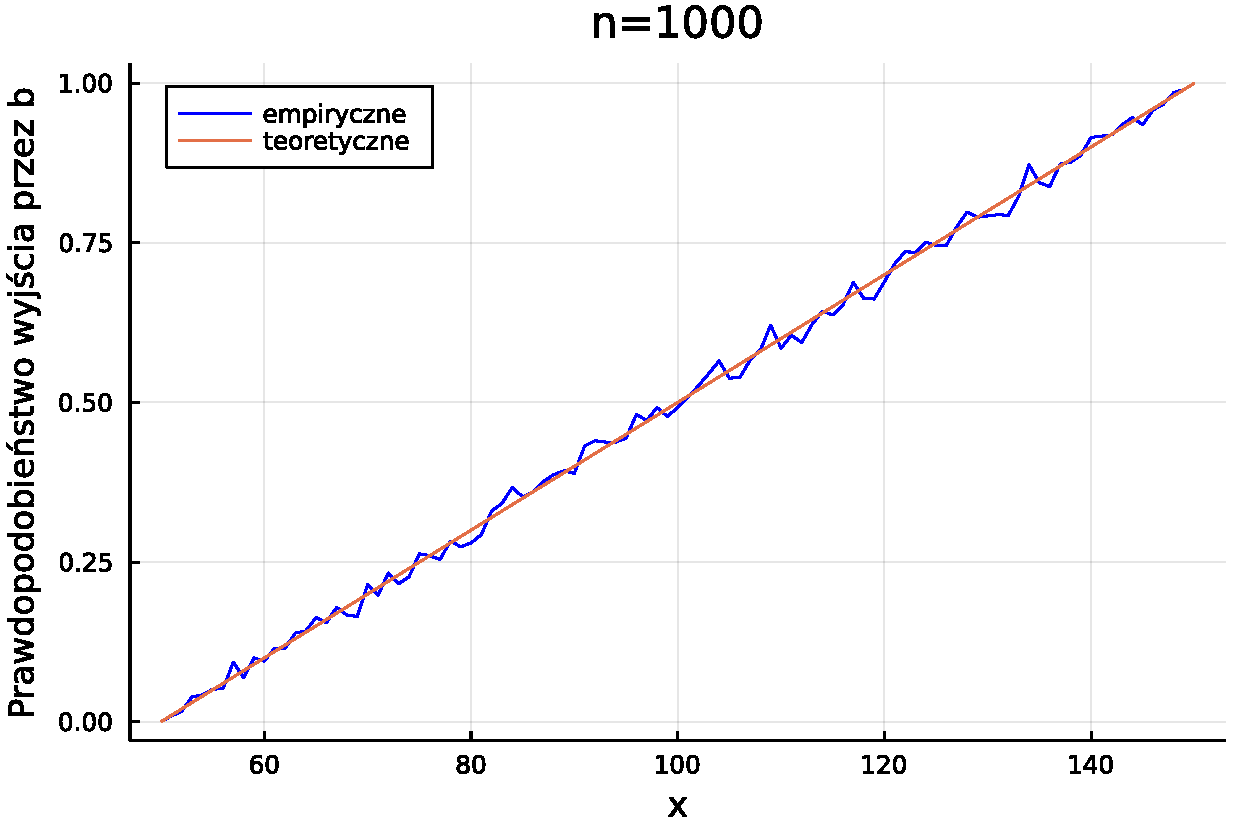
\includegraphics[scale=0.30]{prob100poly.pdf}
			\caption{}
			\label{fig:77}
			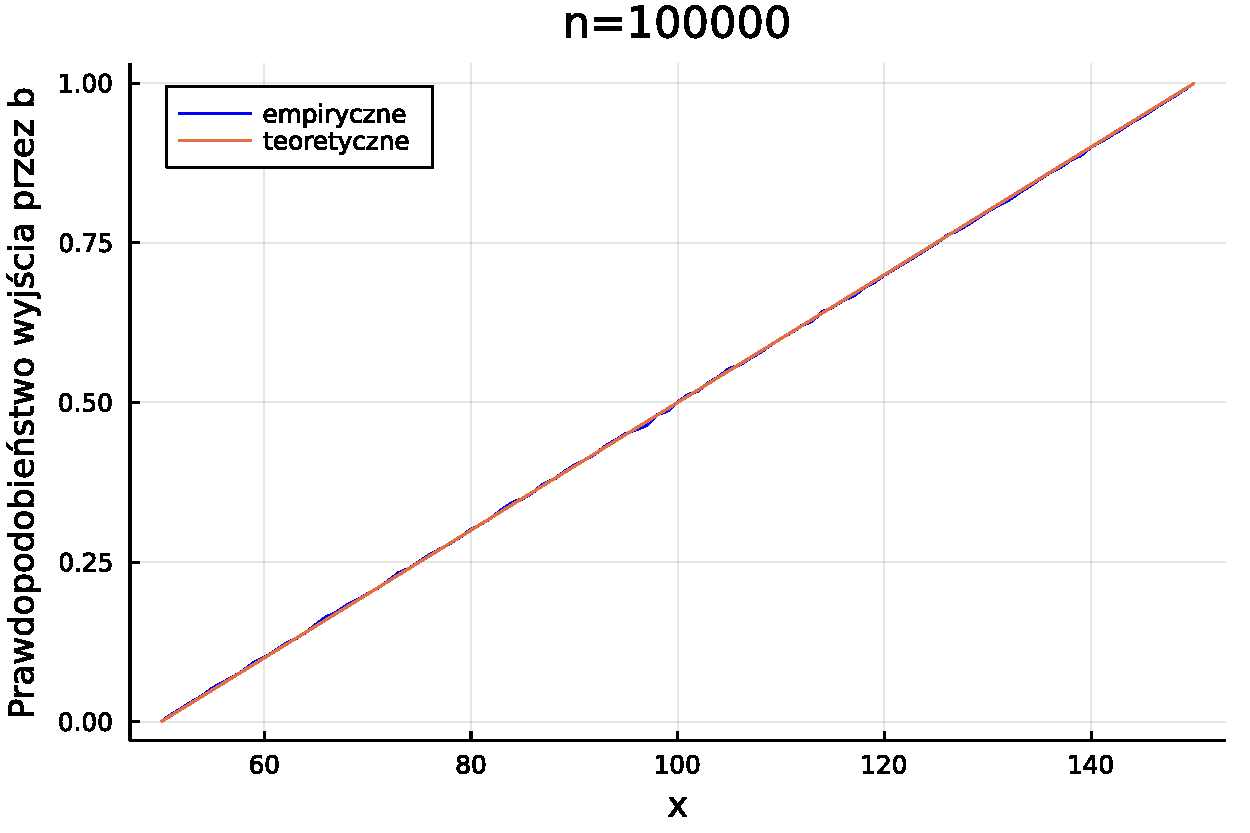
\includegraphics[scale=0.30]{prob100000poly.pdf}
			\caption{}
			\label{fig:88}
		\end{center}
	\end{multicols}
\end{figure}

\subsection*{Podsumowanie}
W zadaniu szukaliśmy zależności między średnim czasem wyjścia z przedziału $[a,b]$ oraz prawdopodobieństwem, że wyjście to nastąpi przez $b$, a wartością początkową $x$. Musimy jednak pamiętać, że przeprowadzając symulację metodą numeryczną, dostaniemy jedynie przybliżone zachowanie procesu Wienera. Aby uzyskać rzeczywisty efekt, nasz minimalny krok czasowy $dt$ musiałby dążyć do zera. Żeby wyniki były jak najbardziej rzetelne, musi zostać spełniony następujący warunek:
 $$dt<<|a-b|.$$ 
Należy jednak pamiętać, że dla ustalonego $dt$, zwiększając różnicę $|a-b|$, zwiększa się również czas wykonywania symulacji, dlatego mając ograniczone warunki, nie powinna być ona zbyt duża. Wykonując więcej powtórzeń $n$, również poprawiamy dokładność otrzymanych wyników, jednak tutaj równie dobrze jest zachować umiar.
\\ \\
Obserwując średni czas wyjścia, w zależności od początkowego $x$, widzimy że rośnie on wraz z odległością do bliższej granicy $a$ lub $b$. Będzie on najdłuższy, kiedy $|x-a|=|x-b|$, czyli dla $x=\frac{a+b}{2}$. Wtedy też prawdopodobieństwo wyjścia przez granicę $b$ jest równe prawdopodobieństwu wyjścia przez granicę $a$:
 $$P(B_{\tau^x}^x=b) = P(B_{\tau^x}^x=a) = \frac{1}{2}$$
Ogólnie:
 $$P(B_{\tau^x}^x=b) = 1 - P(B_{\tau^x}^x=a).$$
\begin{thebibliography}{9}

\bibitem{R. M. Dudley} R.M.Dudley - The Dvoretzky-Kiefer-Wolfowitz inequality with sharp constant - massarts 1990 proof.
\bibitem{goodnes} Goodness of-Fit Techniques, edited by Ralph B. D'Agostimo and Michael A.Stephens, p.97-101.
\bibitem{burnecki} Cížek, Härdle, Weron - Statistical Tools for Finance and Insurance, p.307
\bibitem {polyfit} Dokumentacja funkcji \emph{numpy.polyfit} \url{https://numpy.org/doc/stable/reference/generated/numpy.polyfit.html.}

\end{thebibliography}
\end{document}